\documentclass[12pt]{article}

\usepackage{booktabs}% http://ctan.org/pkg/booktabs
\usepackage[utf8]{inputenc}
\usepackage{changepage}
\usepackage{pgfplots}
\usepackage{amssymb}
\usepackage{xcolor}
\usepackage{hyperref}
\usepackage{listings}
\usepackage[T1]{fontenc}
\usepackage[utf8]{inputenc}
\usepackage{adjustbox}
\usepackage{amsmath}
\usepackage{mathtools}
\usepackage{biblatex}
\usepackage{algorithm2e}
\RestyleAlgo{ruled}
\SetKwProg{Proc}{Procedure}{:}{}


\lstset{
  language=Python,
  numbers=left,
  numberstyle=\tiny,
  stepnumber=1,
  numbersep=5pt,
  tabsize=4,
  basicstyle=\ttfamily,
  columns=fullflexible,
  keepspaces,
}
\hypersetup{
    colorlinks,
    citecolor=black,
    filecolor=black,
    linkcolor=black,
    urlcolor=black
}

% Set page size and margins
% Replace `letterpaper' with `a4paper' for UK/EU standard size
\usepackage[letterpaper,top=2cm,bottom=2cm,left=3cm,right=3cm,marginparwidth=1.75cm]{geometry}

% Useful packages
\usepackage{amsmath}
\usepackage{mathtools}
\usepackage{graphicx}
\newenvironment{para}{\begin{adjustwidth}{13mm}{}}{\end{adjustwidth}}

\newcommand\tab[1][1cm]{\hspace*{#1}}

\newcommand{\tabitem}{\llap{\textbullet}}
\newcommand{\Hsquare}{%
\text{\fboxsep=-.2pt\fbox{\rule{0pt}{1ex}\rule{1ex}{0pt}}}%
}

\newtheorem{Definizione}{Definizione}[subsection]
\newtheorem{Lemma}{Lemma}[subsection]
\newtheorem{Teorema/Definizione}{Teorema/Definizione}[subsection]
\newtheorem{Corollario}{Corollario}[subsection]
\newtheorem{Teorema}{Teorema}[subsection]
\newtheorem{Proposizione}{Proposizione}[subsection]
\newtheorem{Notazione}{Notazione}[subsection]
\newtheorem{Commento}{Commento}[subsection]
\newtheorem{Dimostrazione}{Dimostrazione}[subsection]
\newtheorem{Osservazione}{Osservazione}[subsection]
\newtheorem{Nota}{Nota}[subsection]

\DeclarePairedDelimiter\ceil{\lceil}{\rceil}
\DeclarePairedDelimiter\floor{\lfloor}{\rfloor}


\title{Introduzione all'intelligenza artificiale}
\author{spitfire}
\date{A.A. 2024-2025}
\begin{document}
\begin{figure}
    \centering
    
\includegraphics[width=0.35\textwidth]{Images/Logo scienze bicocca.png}
\end{figure}

\vspace{10cm}
\date{A.A. 2024-2025}


\maketitle

\newpage

\tableofcontents
\newpage

\section{Introduzione}
Che cos'è l'intelligenza artificiale? Prima di tutto, dovremmo definire che cos'è \textbf{l'intelligenza}.
Negli anni sono state date molte definizioni:
\begin{itemize}
    \item "L'intelligenza è una capacità mentale molto \textbf{generale} che, tra le altre cose, coinvolge la capacità di \textbf{ragionare, pianificare, risolvere problemi, pensare in maniera astratta, comprende idee complesse, apprendere velocemente e imparare dall'esperienza}".
     da "Mainstream science on intelligence: An editorial with 52 signatories, history,
        and bibliography, Intelligence 24(1):13–23, 1997"
    \item "L'intelligenza è la \textbf{capacità di adattarsi efficacemente all'ambiente}, o cambiando se stessi o cambiando l'ambiente oppure trovandone uno nuovo... l'intelligenza non è un singolo processo mentale, ma piuttosto una combinazioni molti processi mentali indirizzati verso un adattamento efficace all'ambiente" da Encyclopedia Britannica, 2006.
    \item ... 
\end{itemize}
Quindi il problema di fondo è quello di \textbf{definire l'intelligenza}. Le relazioni tra l'informatica e le scienze cognitive non sono quindi
sporadici e sono particolarmente significativi. Uno schema proposto da \textbf{Russel e Norvig e il seguente}:
\begin{center}
    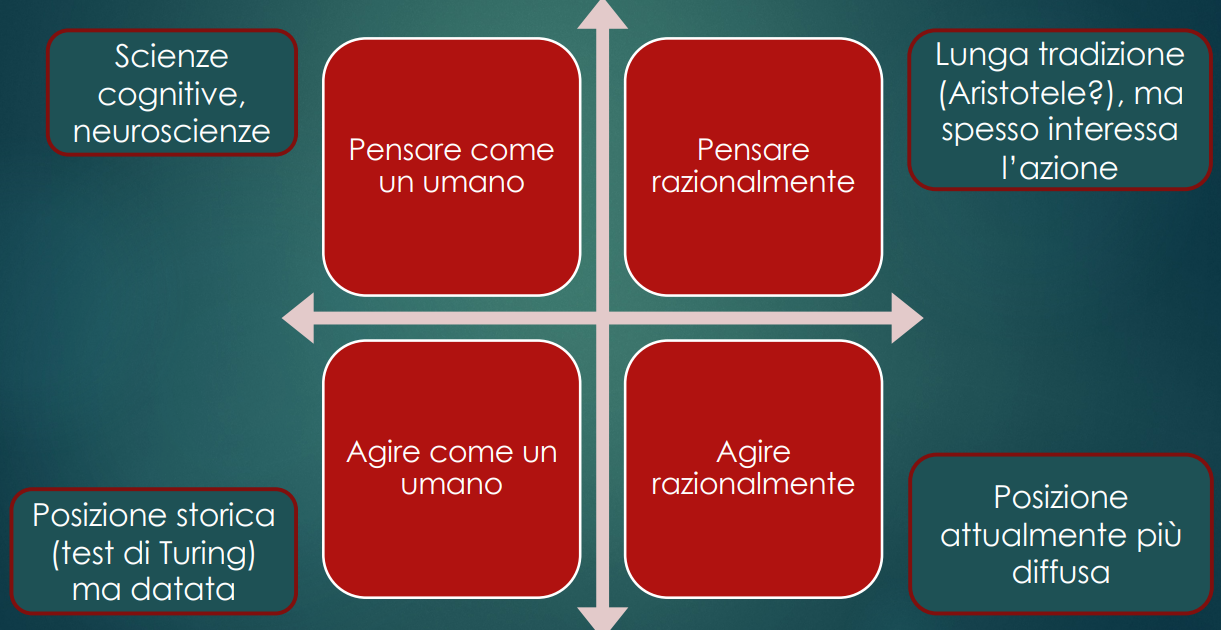
\includegraphics[width = 1\linewidth]{Images/1.PNG}
\end{center}
essi propongono uno schema che "astrae" i tipi di intelligenza, ponendoli su due dimensioni:
\begin{itemize}
    \item Sull'asse delle ordinate troviamo il contrasto tra \textbf{l'imitare l'essere umano} (cioè imitare il suo modo di agire) e il \textbf{pensare come un umano} (quindi il "risolvere problemi")
    \item Sull'asse delle ascisse troviamo il \textbf{contrasto tra il pensare e l'agire}
\end{itemize}
\subsection{Storia dell'intelligenza artificiale}
Il termine "intelligenza artificiale" fu coniato nell'agosto del 1955 da \textbf{John McCarty, Marvin Minsky, Allan Newell e Herbert Simon}, i quali proposero al Dartmouth College di Hanover (New Hampshire) di organizzare il "Dartmouth College Summer Research Project on Artificial Intelligence"; cioè uno spazio
dove accogliere persone che volessero discutere del tema dell'intelligenza artificiale. Essi descrissero l'iniziativa nel seguente modo:
\begin{center}
    "Lo studio dovrà procedere sulla base della congettura che ogni aspetto dell'apprendimento o ogni altra caratteristica dell'intelligenza può essere sia, in linea di principio, descrivibile in maniera talmente precisa che una macchina può essere costruita per simularla"
\end{center} 
In realtà, la storia dell'intelligenza artificiale risale persino ad Alan Turing (1912-1954), il quale definì il cosiddetto \textbf{Test di Turing}: l'idea di questo test è che ci sia un essere umano $C$ separato fisicamente da due interlocutori, uno anch'esso umano, chiamato $B$, e l'altro una macchina, chiamata $A$, programmata in qualche modo.
$C$ non può interloquire direttamente con $A$ e $B$, tuttavia può scambiare messaggi con essi tramite un qualche sistema di comunicazione (foglietti di carta, una chat ecc...). Quando $C$, interagendo in maniera dialogica con i due interlocutori, non riesce più di una certa percentuale di volte a capire chi dei due è la macchina allora $A$ mostra un
comportamento intelligente (cioè "agisce come un essere umano", "agisce razionalmente").
\begin{center}
    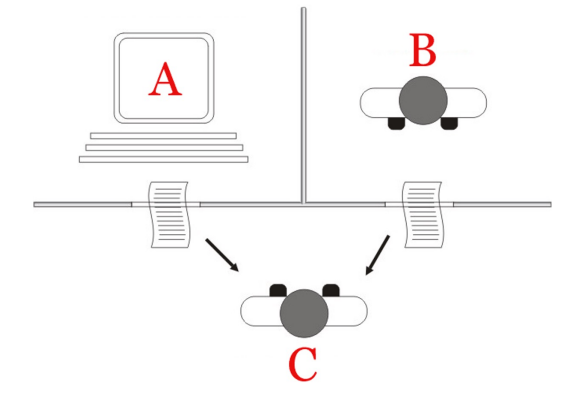
\includegraphics[width = 0.50\linewidth]{Images/2.PNG}
\end{center}
Tuttavia, nel 1966, fu prodotto un programma chiamato \textbf{ELIZA}, il quale imitava uno \textbf{psicoterapeuta}, che \textbf{superò il test di Turing nonostante fosse basato su regole di pattern matching con espressioni regolari}. Il programma portava l'utente ad avere una
\textbf{conversazione plausibile}, cioè davano all'utente l'illusione di star parlando con un \textbf{essere umano}. Per questo, il test di Turing ha solo un \textbf{interesse storico} e risulta poco interessante.
Non è quindi un caso che, nel gruppo di studio citato sopra, una delle cose di cui ci si è occupati non fosse dedicata subito all'apprendimento ma al \textbf{ragionamento}.
\subsection{Approcci simbolici}
La disciplina che si occupa delle forme corrette di ragionamento è la \textbf{logica}.
La logica è quindi lo studio sistematico delle \textbf{forme di inferenza valida}, cioè forme di elaborazione e rappresentazione della conoscenza
che garantiscono che da informazioni vere si derivino informazioni vere.
La \textbf{logica computazionale} è l'uso della logica per effettuare ragionamenti riguardo alla computazione (es. dimostrazione della correttezza di un programma).
Alcuni sforzi iniziali nel settore dell'intelligenza artificiale erano legati alla realizzazione di \textbf{dimostratori automatici di teoremi}. \newline 
Un'\textbf{inferenza} è un ragionamento che stabilisce delle relazioni tra \textbf{premesse} e delle \textbf{conclusioni}. I \textbf{modelli computazionali} di inferenza si interessano quindi di:
\begin{itemize}
    \item Quali informazioni possono trarre dato un insieme di premesse?
    \item Perché la conclusione è corretta?
\end{itemize}
L'inferenza riguarda quindi il trarre delle conclusioni quando \textbf{le premesse sono vere}.
Dire che un'inferenza è corretta, tuttavia, \textbf{non dice nulla sul valore di verità delle conclusioni}, quindi un ragionamento può essere corretto anche se \textbf{le premesse sono false}.
Le varie forme di inferenza sono:
\begin{itemize}
    \item \textbf{Deduzione}:"Se le premesse sono vere, allora le conseguenze devono essere anch'esse vere". Questa forma di ragionamento parte da delle premesse \textbf{generali} e trae delle conclusioni \textbf{particolari}
    \item \textbf{Inferenze di "senso comune"}: Esse non sono sempre "valide", ma sono \textbf{utili nella pratica}; sono modelli per spiegare \textbf{quando un inferenza è giustificata} e calcolarla di conseguenza. Esempi di questo tipo di inferenze sono:
    \begin{itemize}
        \item \textbf{Induzione}: Questa forma di ragionamento parte da delle \textbf{osservazioni particolari} e arriva a delle \textbf{conclusioni generali}.
        \item \textbf{Abduzione}: Sillogismo in cui la premessa maggiore è certa e la premessa minore è probabile, per cui anche la conclusione risulta solo probabile.
    \end{itemize}
\end{itemize}
Dove si applica quindi l'IA di tipo simbolico?
\begin{itemize}
    \item Problemi che possono essere espressi in termini di \textbf{vincoli} che devono essere soddisfatti
    \item Situazioni in cui si devono studiare delle \textbf{sequenze di azioni} per portare un certo stato dell'ambiente circostante ad un determinato obbiettivo
\end{itemize}
In passato, si svilupparono applicazioni il cui obbiettivo era \textbf{risolvere problemi specifici e delimitati}; questa applicazioni presero il nome di \textbf{sistemi esperti}.
Degli esempi notevoli sono:
\begin{itemize}
    \item \textbf{Dendral}(Anni '60): Automatizzò il processo di decisione e l'approccio alla risoluzione dei problemi dei chimici organici
    \item \textbf{Mycin}(Anni '70): Supportò  l'identificazione dei batteri che causavano infezioni gravi e la raccomandazione di antibiotici 
\end{itemize}
\begin{center}
    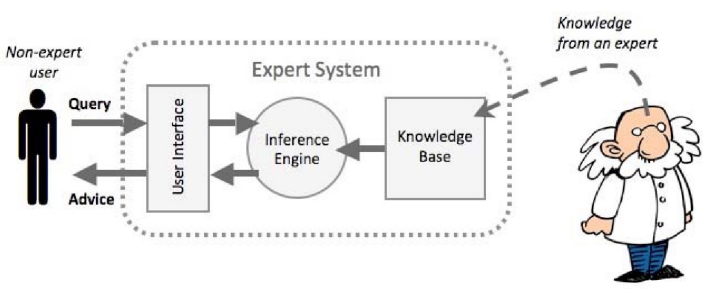
\includegraphics[width = 0.80\linewidth]{Images/3.PNG}
\end{center}
Tuttavia, presto divennero evidenti i \textbf{limiti} dei sistemi esperti:
\begin{itemize}
    \item È necessario trovare un \textbf{esperto disposto a codificare la sua conoscenza all'interno della base di conoscenza}
    \item I sistemi esperti \textbf{non scalano bene con grandi quantità di informazioni}: l'aggiornamento del sistema esperto rispetto ai \textbf{nuovi approcci alla risoluzione del problema per cui è stato costruito} è particolarmente complesso, sopratutto se il problema \textbf{non è ben delimitato}. La base di conoscenza del sistema rischierebbe quindi di \textbf{contenere troppi assiomi e regole}.
    \item Il costo di sviluppo di questi sistemi è \textbf{elevato}
\end{itemize}
\subsection{Approcci sub-simbolici}
I sistemi di IA \textbf{sub-simbolici} \textbf{non manipolano una rappresentazione simbolica} per trovare soluzioni a problemi, ma effettuano \textbf{calcoli secondo alcuni principi} che hanno dimostrato di essere in grado di portare alla risoluzione del problema.
Esempi notevoli sono:
\begin{itemize}
    \item Algoritmi genetici
    \item Reti Neurali
    \item "Intelligenza dello sciame" (Swarm Intelligence)
\end{itemize}
Tuttavia, l'argomento più importante correntemente è quello del \textbf{Machine Learning}.
Le \textbf{reti neurali artificiali} (Artificial Neural Networks (ANN)) sono una simulazione astratta del nostro sistema nervoso, il quale
contiene una collezione di \textbf{neuroni} che comunicano tra loro tramite delle connessioni dette \textbf{assoni}.
\begin{center}
    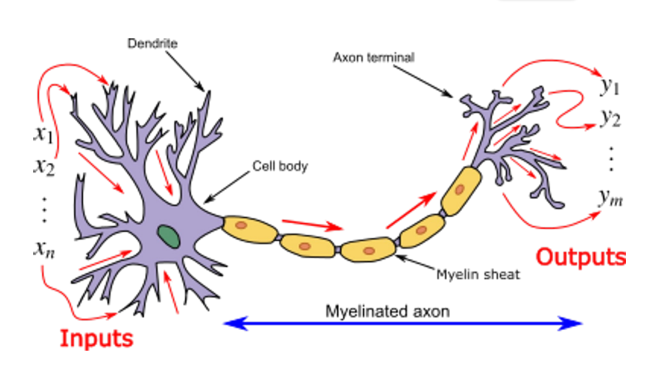
\includegraphics[width = 0.60\linewidth]{Images/4.PNG}
\end{center}
Il modello delle ANN ha delle certe somiglianze con gli assoni e i dendriti nel nostro sistema nervoso.
Il primo modello di rete neurale artificiale fu proposto nel 1943 da \textbf{McCulloch} e \textbf{Pits} nei termini di un \textbf{modello computazione dell'attività neurale}.
Questo modello fu poi seguito da altri modelli proposti da \textbf{John Von Neumann, Marvin Minsky, Frank Rosenblatt} e molti altri.
Rosenblatt definì un modello "algebrico" del neurone, chiamato \textbf{percettrone}; esso è una pietra miliare della ricerca sulle reti neurali.
Il percettrone cerca di \textbf{simulare le operazioni svolte da un singolo neurone}; l'apprendimento quindi diventa un problema di \textbf{scegliere i pesi e le soglie corrette}.
\begin{center}
    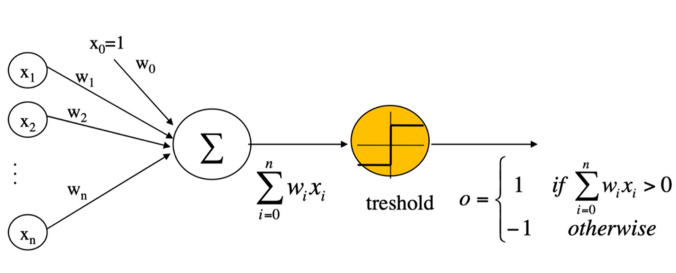
\includegraphics[width = 0.70\linewidth]{Images/5.PNG}
\end{center}
tendenzialmente, si arriva ad avere dei \textbf{percettroni multistrato}, dove ogni nodo è un singolo percettrone (introdotti per la prima volta da Minksy e S.Papert nel 1969)
\begin{center}
    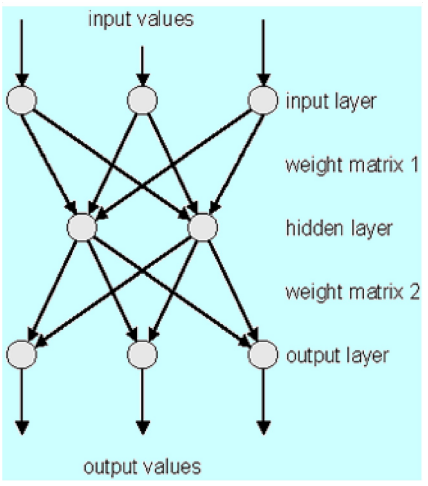
\includegraphics[width = 0.40\linewidth]{Images/6.PNG}
\end{center}
come faccio però a determinare i pesi di tutta la rete? Si utilizza il meccanismo della \textbf{back-propagation}: l'idea è che l'input è una \textbf{rappresentazione del problema} e che vi sia un \textbf{output desiderato} che la rete deve offrire;
inizialmente la rete neurale ha \textbf{dei pesi causali}, che verranno corretti \textbf{retropropagando} l'output desiderato sulla rete.
Questo è un approccio all'apprendimento che si dice "\textbf{supervisionato}".
\begin{center}
    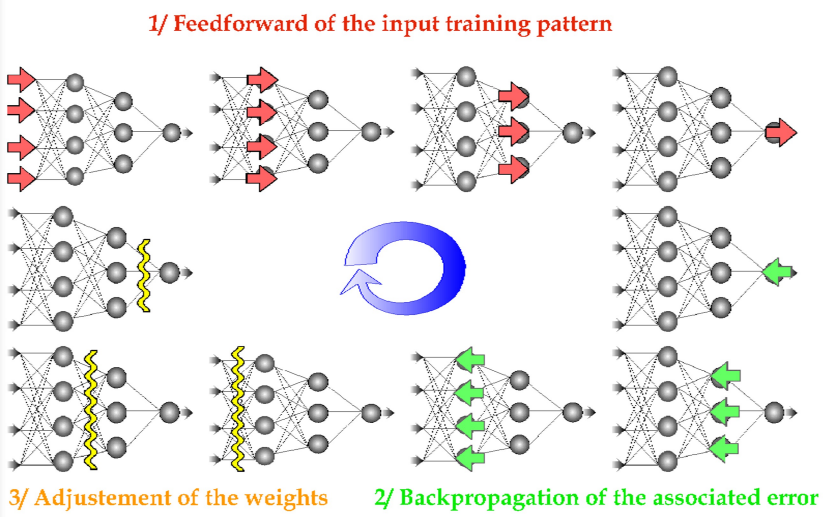
\includegraphics[width = 0.75\linewidth]{Images/7.PNG}
\end{center}
Oltre all'apprendimento supervisionato, esistono molte altre tecniche di addestramento:
\begin{center}
    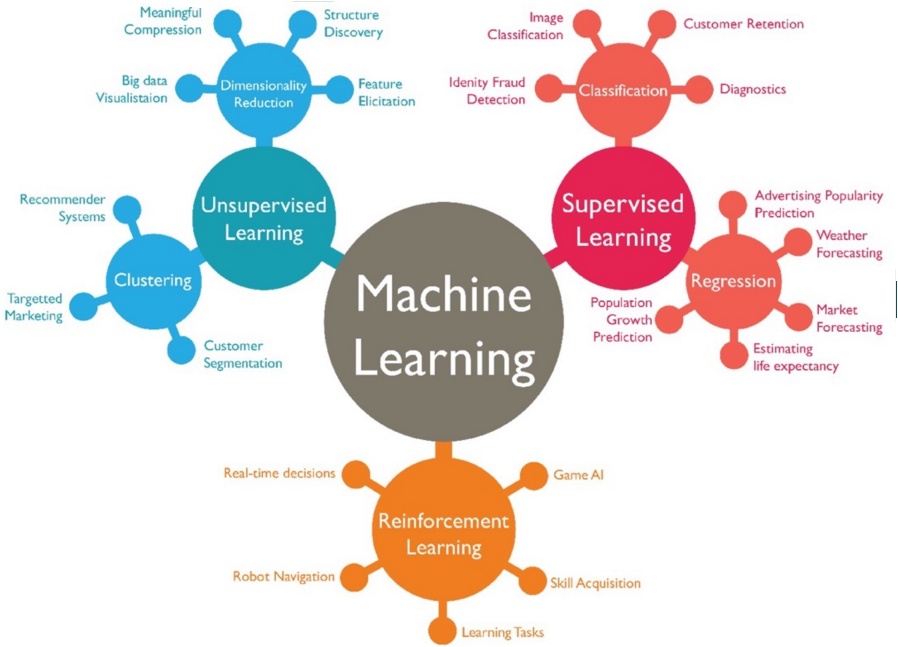
\includegraphics[width = 0.95\linewidth]{Images/8.PNG}
\end{center}
\newpage
\subsection{Agenti intelligenti, architetture e ambienti}
Un \textbf{agente} è tutto ciò che può essere vista come "percepente il suo ambiente" attraverso dei \textbf{sensori} e che può \textbf{agire su tale ambiente} attraverso degli \textbf{attuatori}.
Come agenti possono essere quindi classificati
\begin{itemize}
    \item Gli \textbf{esseri umani}, definendo come "sensori" gli occhi, le orecchie ecc... e come attuatori la bocca, le gambe, le braccia ecc...
    \item Gli \textbf{agenti robotici}, i quali hanno telecamere e sensori ad infrarossi come sensori e vari motori come attuatori
    \item Nulla vieta che \textbf{un agente possa essere anche solamente un software}
\end{itemize} 
Un agente è quindi rappresentabile nel seguente modo:
\begin{center}
    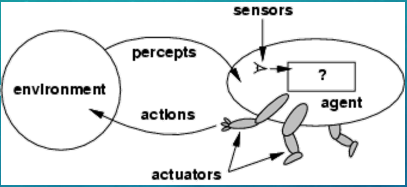
\includegraphics[width = 0.45\linewidth]{Images/9.PNG}
\end{center}
la forma più generale di agente è una \textbf{funzione} che mappa \textbf{l'insieme potenza di tutte le percezioni istantanee $\mathcal{P}^*$} ad una azione dell'insieme \textbf{di tutte le azioni eseguibili dall'agente} $\mathcal{A}$, cioè:
$$f: \mathcal{P}^* \rightarrow \mathcal{A}$$
quindi, l'agente può mappare una \textbf{sequenza arbitrariamente lunga di percezioni istantanee} (insieme potenza di $\mathcal{P}$) \textbf{ad una singola azione contenuta nell'insieme $\mathcal{A}$}.
Un agente è quindi \textbf{la sua architettura (la sua struttura profonda) più il suo programma (specifico dell'agente)}.
Gli agenti possono essere classificati, in base alla loro architettura interna, nelle seguenti classi:
\begin{itemize}
    \item Agenti con riflessi semplici
    \item Agenti con riflessi basati su un modello
    \item Agenti basati su un obbiettivo e su un modello
    \item Agenti basati su un'utilità e un modello.
\end{itemize}
\subsubsection{Agenti con riflessi semplici}
Un agente con riflessi semplici è un agente in cui vi è una comunicazione con l'ambiente (tramite i sensori e gli attuatori dell'agente).
Al suo interno, i sensori vanno a realizzare una "vista" che rappresenta \textbf{lo stato attuale dell'ambiente circostante}.
L'agente deve quindi \textbf{scegliere quale azione intraprendere} e, in questo caso, per farlo ha solamente a disposizione delle regole del tipo
\textbf{condizione-azione}.
\begin{center}
    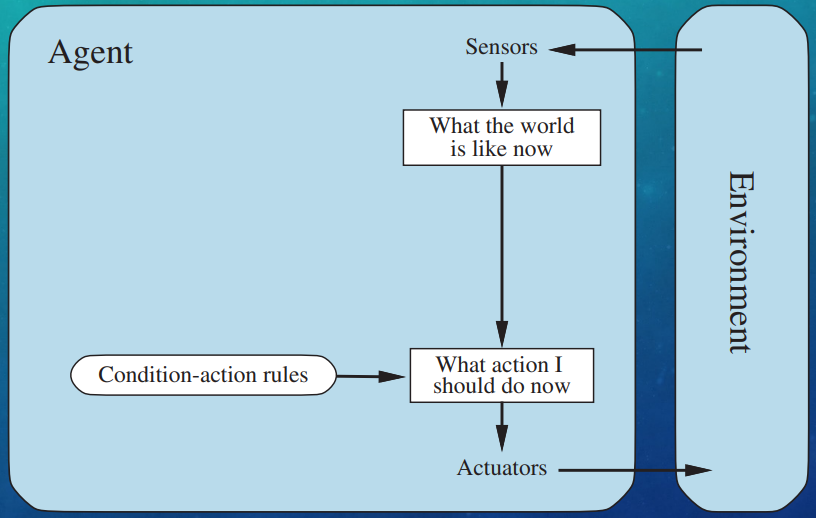
\includegraphics[width = 0.70\linewidth]{Images/10.PNG}
\end{center}
questo tipo di agente è \textbf{privo di stato}. Con architetture estremamente semplici, magari con più agenti, si riescono
quindi ad ottenere dei comportamenti, se non intelligenti, perlomeno utili.
\subsubsection{Agenti con riflessi basati su modello}
\begin{center}
    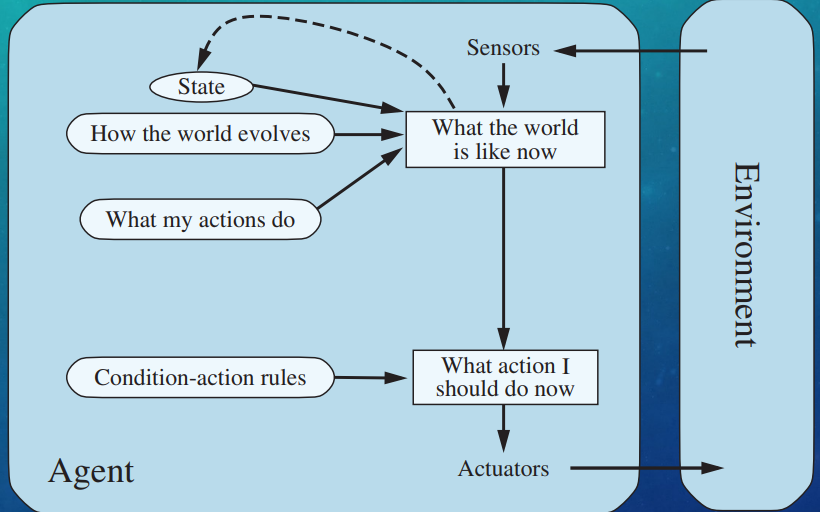
\includegraphics[width = 0.70\linewidth]{Images/11.PNG}
\end{center}
La differenza più significativa di questi agenti rispetto agli agenti con riflessi semplici è la \textbf{conoscenza del proprio stato interno}.
Questo tipo di agente può quindi \textbf{riflettere sul proprio stato} e quindi effettuare azioni basate su di esso.
Anche ignorando che l'ambiente ha una struttura, questo tipo di agente deve quindi avere un \textbf{modello matematico dell'evoluzione del mondo rispetto alle azioni fatte} che gli permetta
di decidere quale azioni intraprendere. Lo stato \textbf{non è una memoria che mantiene lo stato del mondo}, ma è solo un'informazione sullo stato dell'agente.
L'agente, inoltre, deve \textbf{poter percepire il proprio stato come parte dell'ambiente} (o come una "percezione esterna" o proprio come uno stato interno all'agente e che esso aggiorna e conosce).
Questo tipo di agente quindi può eseguire \textbf{comportamenti più adattivi rispetto all'ambiente}.
\subsubsection{Agenti basati su un obbiettivo e su un modello}
\begin{center}
    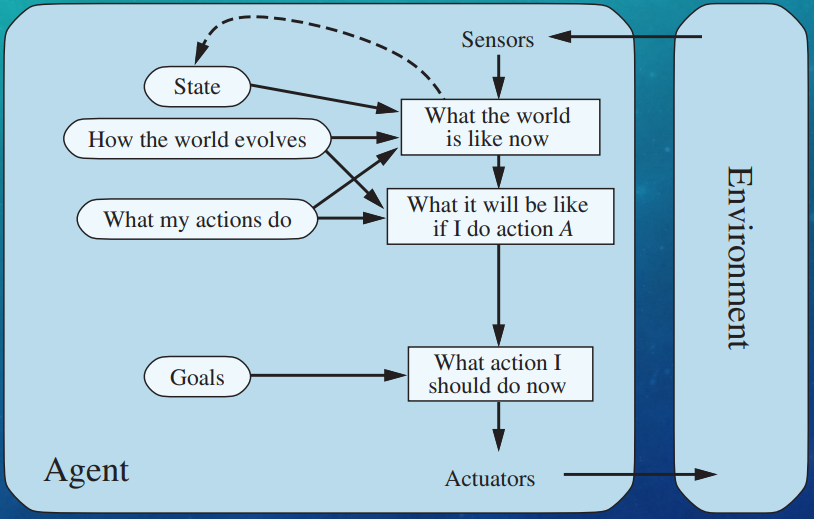
\includegraphics[width = 0.70\linewidth]{Images/12.PNG}
\end{center}
Questo tipo di agente, tramite i sensori ed eventualmente l'informazione di stato, si fa un'idea dello stato in cui si trova.
Questo agente presenta una \textbf{funzione che, partendo dallo stato dell'agente, ritorna tutte le azioni ammissibili che l'agente può intraprendere}.
Lo stato attuale viene quindi messo come \textbf{radice di un albero} e generiamo, a partire da esso, un numero di figli pari al numero di azioni ammissibili.
Possiamo costruire questo albero perché sappiamo \textbf{in quale stato si andrà a finire eseguendo una determinata azione}.
Per ogni nodo di stato che viene generato in questo modo, potremmo generare \textbf{un ulteriore livello di approfondimento dell'albero}, cioè ogni nodo stato potrebbe diventare la radice di un ulteriore sotto-albero.
In linea di principio, potrei quindi costruire l'albero di \textbf{tutti gli stati raggiungibili possibili tramite ogni combinazione possibile di azioni}.
Ovviamente, il fattore di ramificazione di questo albero è \textbf{estremamente elevato}. L'agente deve quindi esplorare questo albero per capire se esistono delle configurazioni nelle quali \textbf{l'obbiettivo sia verificato}.
Vi è quindi una \textbf{costruzione dello spazio degli stati} e una \textbf{ricerca nello spazio degli stati}. \newline
Per capire quali azioni intraprende, l'agente deve quindi risolvere un \textbf{problema di ricerca}, il quale consiste in:
\begin{itemize}
    \item Uno \textbf{spazio degli stati}
    \item Una \textbf{funzione di successione}, che dato un certo stato e l'azione che si vuole intraprendere (la quale potrebbe avere un certo \textbf{costo}), in quale stato si vada a finire. Questa funzione mi dice anche \textbf{quali sono le azioni ammissibili in un determinato stato}
    \item Uno \textbf{stato iniziale}
    \item Una \textbf{funzione "goal test"} che ci dica \textbf{se l'obbiettivo è stato raggiunto o meno}
\end{itemize}
Una \textbf{soluzione} ad un problema di ricerca è una \textbf{sequenza di azioni} (un piano) che trasformano lo stato iniziale nello stato obbiettivo.
Uno \textbf{spazio di ricerca} astrae l'ambiente per selezionare solo le informazioni utili per risolvere il problema.
\begin{center}
    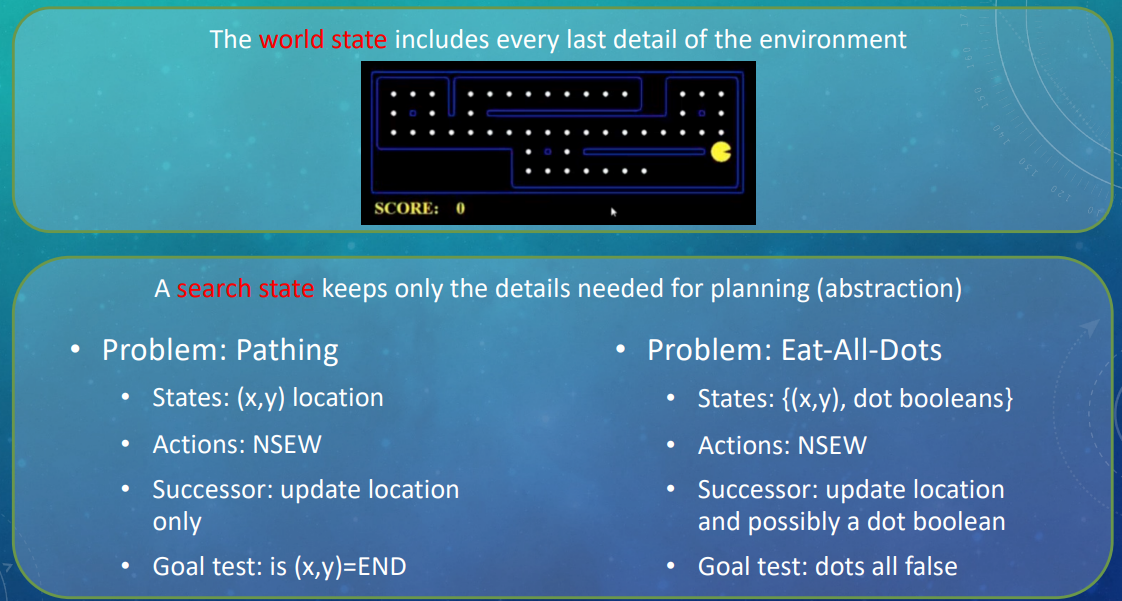
\includegraphics[width = 1\linewidth]{Images/13.PNG}
\end{center}
lo spazio degli stati, per problemi di ragionevole complessità, \textbf{tendono ad esplodere}, quindi non si possono applicare generalmente algoritmi \textbf{forza bruta} per trovare una configurazione che risolva il problema.
La costruzione dello spazio di ricerca avviene tramite \textbf{un albero di ricerca}, dove:
\begin{itemize}
    \item Lo stato iniziale è il nodo radice
    \item I figli corrispondono agli stati successivi data un'azione
    \item I nodi mostrano gli stati, ma \textbf{corrispondono ai piani per raggiungere quelli stati}
    \item Per la maggior parte dei problemi, non arriviamo mai a costruire l'intero albero (troppo grande)
\end{itemize}
\begin{center}
    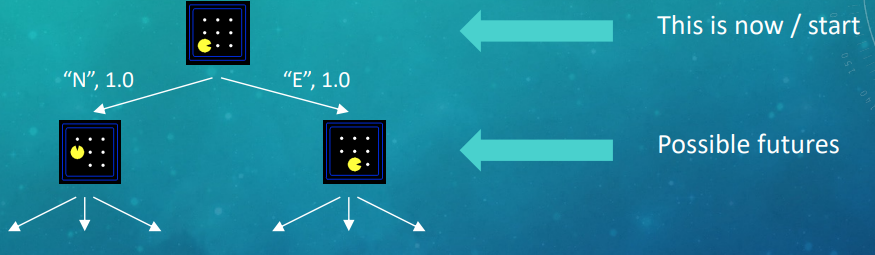
\includegraphics[width = 1\linewidth]{Images/14.PNG}
\end{center}
Invece di usare un albero per rappresentare il problema di ricerca, potremmo invece usare un \textbf{grafo dello spazio degli stati}: esso da una rappresentazione matematica del problema di ricerca nel seguente modo:
\begin{itemize}
    \item I nodi sono \textbf{le possibili configurazioni del mondo}
    \item Gli archi rappresentano \textbf{i risultati delle azioni}
    \item La funzione \textbf{"goal test"} viene rappresentata da un \textbf{insieme di nodi}
\end{itemize}
\begin{center}
    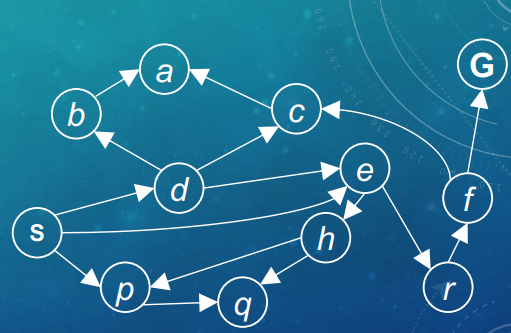
\includegraphics[width = 0.50\linewidth]{Images/15.PNG}
\end{center}
In un grafo dello spazio degli stati, \textbf{ogni stato occorre solamente una volta!} Tuttavia, raramente possiamo costruire l'intero grafo in memoria, poiché \textbf{esso cresce troppo velocemente}; tuttavia è un'idea utile.
Qual'è quindi la differenza sostanziale tra un grafo dello spazio degli stati e un albero di ricerca? Ogni \textbf{nodo} in un albero di ricerca è l'equivalente di un \textbf{intero cammino sul grafo dello spazio degli stati}.
Entrambi devono essere costruiti \textbf{"on demand"} (cioè li espandiamo solamente quando occorre) e devono esser espansi il meno possibile.
\subsubsection{Agenti basati su un'utilità e un modello}
\begin{center}
    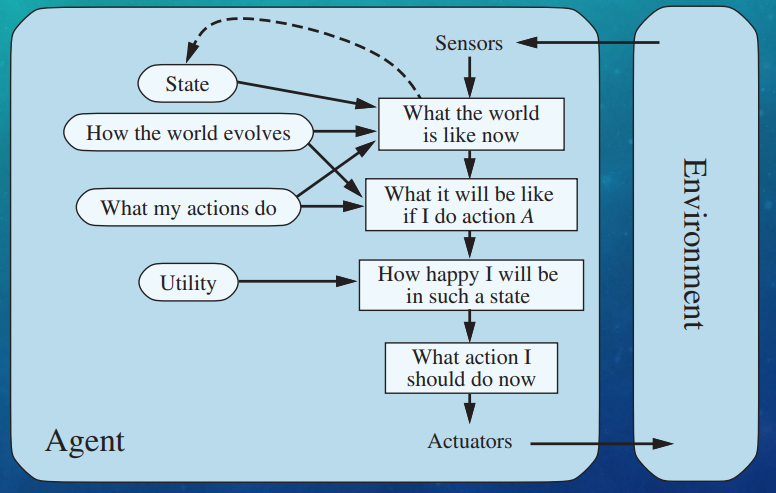
\includegraphics[width = 0.80\linewidth]{Images/16.PNG}
\end{center}
La differenza di questo tipo di agente con il precedente è la \textbf{scomparsa della funzione "goal test"} e l'introduzione di una \textbf{funzione "Utility"}, la quale è una vera e propria funzione
che attribuisce ad un certo stato del mondo un idea di \textbf{quanto quello stato sia desiderabile dall'agente}. Perché? Ci sono diversi motivi:
\begin{itemize}
    \item Potrei non essere in grado di definire formalmente una funzione che descriva l'obbiettivo
    \item Dato lo stato dell'ambiente, posso definire una funzione che valuti i vari elementi di esso e mi permetta di effettuare valutazione sulla prossima aziona da eseguire (es. scacchi)
    \item Avere una funzione d'utilità mi permette di considerare obbiettivi contrastanti fra loro; quindi poter definire una funzione che valuti tutti i fattori in gioco e che possa portare alla \textbf{discriminazione di certi stati} (es. problema di logistica)
\end{itemize}
\subsubsection{Caratteristiche dell'ambiente}
Russel e Norvig definiscono una serie di caratteristiche per l'ambiente:
\begin{itemize}
    \item \textbf{Ambienti accessibili vs Inaccessibili}: Un \textbf{ambiente accessibile} è un ambiente dove l'agente può ottenere un informazione \textbf{completa, accurata e aggiornata} riguardo lo stato dell'ambiente.
    Molti ambiente moderatamente complessi (includendo, per esempio, il mondo fisico e internet) sono \textbf{inaccessibili}. Più un ambiente è accessibile, più è semplice costruire un agente che possa operare in esso.
    I problemi di accessibilità del mondo si presentano ogni qualvolta che ci accingiamo a risolvere problemi nel \textbf{mondo fisico}
    \item \textbf{Ambienti deterministici vs non-deterministici}: Un \textbf{ambiente deterministico} è un ambiente in cui ogni azione ha un singolo effetto garantito: non c'è \textbf{incertezza} riguardo allo stato in cui l'ambiente si troverà in seguito al compiersi di un azione. Il mondo fisico dovrebbe essere sempre considerato come sostanzialmente \textbf{non-deterministico}, salvo certi casi in cui si può pensare come deterministico.
    Gli ambienti non-deterministici presentano problemi maggiore per il progettista dell'agente.
    \item \textbf{Ambienti episodici vs sequenziali}: In un ambiente \textbf{episodico}, l'esperienza dell'agente può essere divisa in \textbf{passi atomici} dove l'agente percepisce uno stimolo ed effettua una singola azione. La scelta dell'azione da intraprendere \textbf{dipende solamente dall'episodio stesso}.
    Gli ambienti episodici sono più semplici dal punto di vista del progettista dell'agente, poiché l'agente può decidere quale azione intraprendere basandosi solo sull'episodio corrente, \textbf{non deve quindi ragionare riguardo all'interazione tra questo episodio e quelli futuri}.
    \item \textbf{Ambienti statici vs dinamici}: Per \textbf{ambiente statico} si intende un ambiente che \textbf{non cambia nel mentre che l'agente sta decidendo l'azione da compiere}; un cambiamento in un ambiente statico avviene quindi \textbf{solamente a causa di un'azione da parte dell'agente}.
    Per \textbf{ambiente dinamico} si intende un ambiente che \textbf{cambia mentre l'agente sta decidendo quale azione intraprendere} e che quindi ha al suo interno altri processi, oltre all'agente, che ne modificano lo stato e le cui azioni possono interferire con le azioni dell'agente (come nella teoria dei sistemi concorrenti); le trasformazioni di un ambiente dinamico quindi avvengono \textbf{al di fuori del controllo dell'agente}.
    Il mondo fisico è un ambiente altamente dinamico.
    \item \textbf{Ambienti discreti vs continui}: Un \textbf{ambiente discreto} è un ambiente che presenta un numero \textbf{fissato e finito} di azioni e di percezioni in esso. Gli \textbf{ambienti continui} hanno un certo livello di \textbf{discrepanza} con i sistemi computerizzati.
    Gli ambienti discreti potrebbero essere gestiti, in linea di principio, da una specie di \textbf{tabella di ricerca} (lookup table).
    Per semplificare la gestione di un ambiente continuo, si può \textbf{sovrapporre ad esso una sua discretizzazione} in modo da rendere più semplice la progettazione e l'implementazione degli agenti che devono operare al suo interno.
\end{itemize} 
\begin{center}
    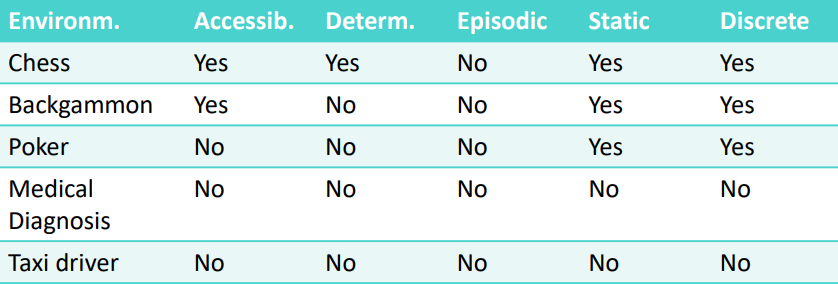
\includegraphics[width = 0.80\linewidth]{Images/17.PNG}
\end{center}
\section{Approcci simbolici - Planning}
Come abbiamo visto, definire in maniera precisa cos'è l'intelligenza è un compito piuttosto complicato.
La ricerca di una definizione univoca ha portato a definizioni di intelligenza \textbf{più focalizzate sulle singole funzioni} e ha portato alla seguente distinzione in termini di performance:
\begin{center}
    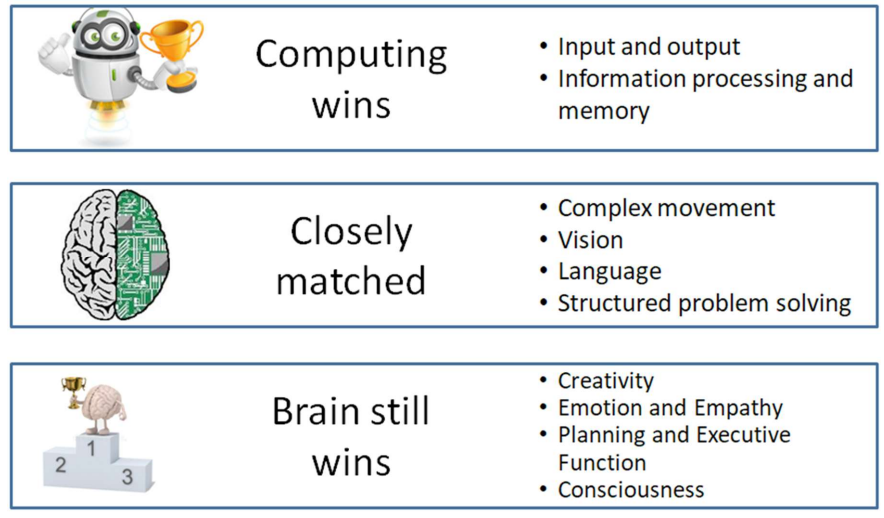
\includegraphics[width = 0.80\linewidth]{Images/18.PNG}
\end{center}
abbiamo quindi dato una definizione di intelligenza basandoci su dei \textbf{compiti da svolgere}, i quali possono essere a volte dei \textbf{problemi}.
Ma quindi, cos'è effettivamente un problema? Possiamo dare la seguente definizione:
\begin{center}
    Vogliamo \textbf{realizzare una condizione desiderata}, che all'inizio non è soddisfatta. Per farlo, dobbiamo \textbf{scegliere} quali azioni intraprendere da un insieme di \textbf{possibili scelte (complesse)}.
\end{center}
Uno degli interessi di studio nel campo dell'intelligenza artificiale è anche quello di \textbf{comprendere come gli essere umani risolvono i problemi}.
Possiamo quindi partire dalla nozione di \textbf{risolutore di problemi generici}, di cui una versione possibile è la seguente:
\begin{center}
    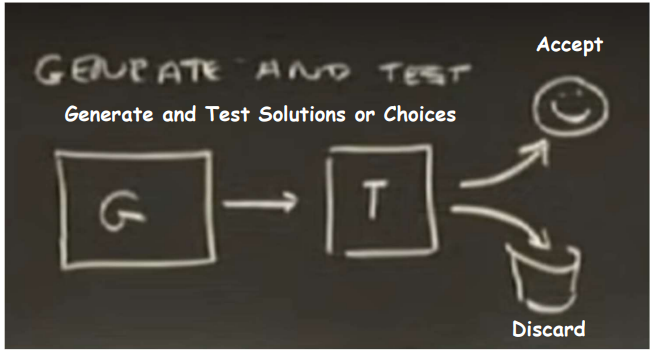
\includegraphics[width = 0.60\linewidth]{Images/19.PNG}
\end{center}
quando questa soluzione può essere inefficiente oppure quando essa può fallire?
\begin{itemize}
    \item Una fonte di inefficienza può essere la \textbf{necessità di effettuare un test su tutte le condizioni generate}
    \item Il costo di una soluzione \textbf{potrebbe essere elevato sia dal punto di vista economico che umano}
    \item Generare le soluzioni ha un costo
    \item Questo sistema può fallire non solo \textbf{quando le possibili scelte sono tante} ma anche quando il generatore \textbf{non riesce a generare tutte le possibili soluzioni oppure esse sono infinite} 
\end{itemize}
nonostante le problematiche sopra, il fatto di \textbf{poter enumerare e valutare tutte le possibili soluzioni al problema} è già un modo di risolverlo quando il suo spazio delle soluzioni (e quindi delle scelte) è limitato.
Ci sono varie condizioni dove si possono applicare, in maniera efficiente, questo tipo di risolutori; alcuni esempi sono:
\begin{itemize}
    \item \textbf{Risolvere puzzle}: In questo caso, la condizione desiderata è \textbf{raggiungere la configurazione base del puzzle} (es. il cubo di rubik con tutte le facce di un certo colore) in una certa maniera (più velocemente? con meno azioni possibili? ecc...)
    La condizione iniziale \textbf{è una configurazione randomica del puzzle}. In questo caso, dobbiamo produrre la sequenza di tutte le azioni necessarie per arrivare alla condizione desiderata rispettando i limiti di tempo/mosse dati.
    Le \textbf{scelte} in questo caso sono \textbf{le sequenza di cambiamenti (complessi) nella configurazione del puzzle}, mentre le \textbf{azioni} sono invece ciò che ci permette di muoverci da una configurazione del puzzle all'altra per creare, concatenandole in sequenza, delle \textbf{scelte} che possano essere valutate rispetto al nostro obbiettivo.
    Ovviamente, per esempio, raggiungere l'obbiettivo con il minor numero di mosse possibili \textbf{non è detto che sia la maniera più veloce} e viceversa.
    \newpage
    \item \textbf{Pacman}:
    \begin{itemize}
        \item \textbf{Condizione desiderata}: mangiare la pillola più vicina? Mangiare tutte le pillole il più velocemente possibile?
        \item \textbf{Inizialmente}: Pacman si trova da qualche parte all'interno del labirinto
        \item \textbf{Scelte}: Strada 1, Strada 2, ..., Strada $N + 1$
        \item \textbf{Azioni}: su, giù, sinistra, destra
    \end{itemize}
    \item ...
\end{itemize}
ciò che hanno in comunque questi esempi è che entrambi presentano delle \textbf{condizioni}, cioè degli \textbf{stati}.
Partendo da una configurazione iniziale e compiendo un'azione, ci troviamo in una configurazione successiva, in cui possiamo compiere
un'altra azione ed arrivare ad un'altra configurazione. L'iterazione di questo processo ci permette di creare \textbf{sequenze di cambiamenti} (le scelte) e quindi di \textbf{generare ogni possibile configurazione del problema}.
Abbiamo quindi ottenuto il generatore $G$ del risolutore sopra.
La possibilità di testare se la configurazione soddisfa l'obbiettivo dipende da come definiamo la configurazione stessa.
Ciò che resta da fare è quindi trovare dei buoni modi per implementare i generatori di soluzioni $G$ e per testare le soluzioni che generano velocemente.
\subsection{Problemi di ricerca}
Come abbiamo visto, le soluzioni possono essere costruite come \textbf{sequenze di stati (o configurazioni e azioni che le cambiano)}.
I tipi di problemi che abbiamo visto sopra si dicono \textbf{problemi di ricerca}, nei quali abbiamo:
\begin{itemize}
    \item Uno \textbf{spazio degli stati} (insieme degli stati) $\mathcal{S}$
    \item Uno \textbf{stato iniziale} $s_0$
    \item Un \textbf{insieme delle azioni possibili in ogni stato} $\mathcal{A}(\mathcal{s})$
    \item Una \textbf{funzione di successione/transizione} $s' = next$
    \item Un \textbf{"goal test"} $G(s)$ che dice se abbiamo raggiunto l'obbiettivo
    \item Un \textbf{costo per ogni azione} $c(s, a, s')$ (opzionale)
    \item 
\end{itemize}
Una \textbf{soluzione ad un problema di ricerca} è una sequenza di azioni (un piano) che trasforma lo stato iniziale in uno \textbf{stato obbiettivo}, cioè in uno stato che soddisfi il \textbf{goal test}.
Una \textbf{soluzione ottimale} ha il \textbf{costo minore tra tutte le possibili soluzioni}.
Lo stato di un problema \textbf{può essere rappresentato in molti modi diversi} (es. pixel, spazio degli stati ecc...).
Per evitare di complicare troppo il problema di ricerca definendo uno spazio degli stati inefficiente, possiamo seguire le \textbf{condizioni di Markov sugli stati, sui successori e sul goal test}:
\begin{itemize}
    \item L'efficienza richiede un \textbf{insieme degli stati il più piccolo possibile}; tuttavia esso deve soddisfare le seguente condizioni:
    \begin{enumerate}
        \item Data una funzione di transizione, uno stato \textbf{contiene tutte le informazioni necessarie per arrivare all'obbiettivo tramite la scelta di azioni da intraprendere}
        \item Dato lo stato $s(t)$, il risultato $s(t+1) = next(s(t), a(t))$ della prossima azione $a(t)$ non dipende dagli stati precedenti $s(t')$ o dalle azioni precedenti
        \item Il goal test può essere applicato direttamente agli stati senza che sia richiesta dell'altra informazione aggiuntiva.
    \end{enumerate}
\end{itemize}
\begin{center}
    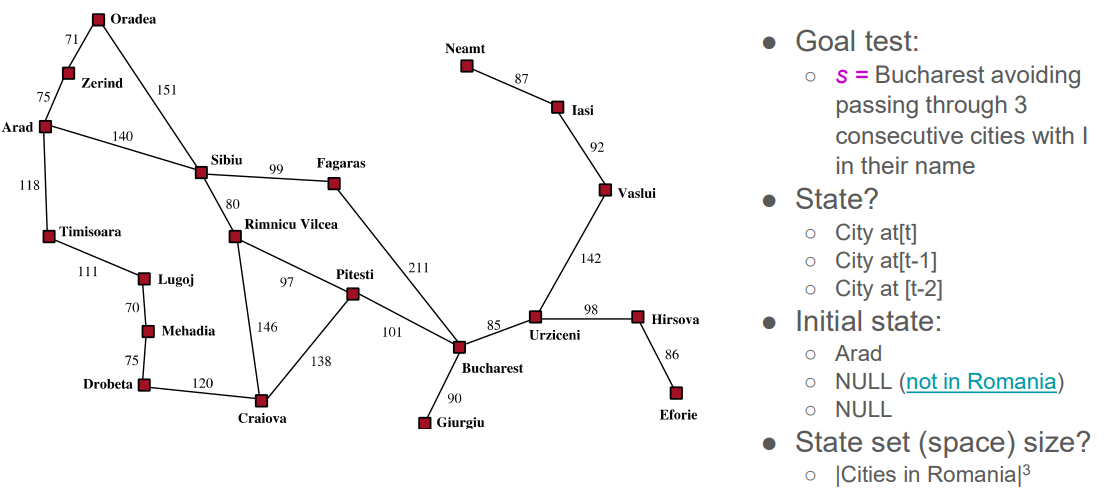
\includegraphics[width = 1\linewidth]{Images/20.PNG}
\end{center}
La condizione in cui risolvere un problema di ricerca risulta più semplice è quando \textbf{il numero degli stati e delle azioni è finito} e \textbf{per ogni azione, c'è un solo possibile stato di destinazione che si raggiunge}.
Per risolvere un problema con la ricerca, ciò che possiamo fare è quindi generare \textbf{tutte le configurazioni a cui le azioni possibili in un certo stato $s$ portano} e poi scegliere quali
di esse espandere ulteriormente. La scelta di \textbf{quale configurazione espandere determina il comportamento dell'agente durante la risoluzione del problema} (esso, per esempio, potrebbe anche entrare in un loop infinito).
Facciamo un esempio: dato il seguente problema:
\begin{center}
    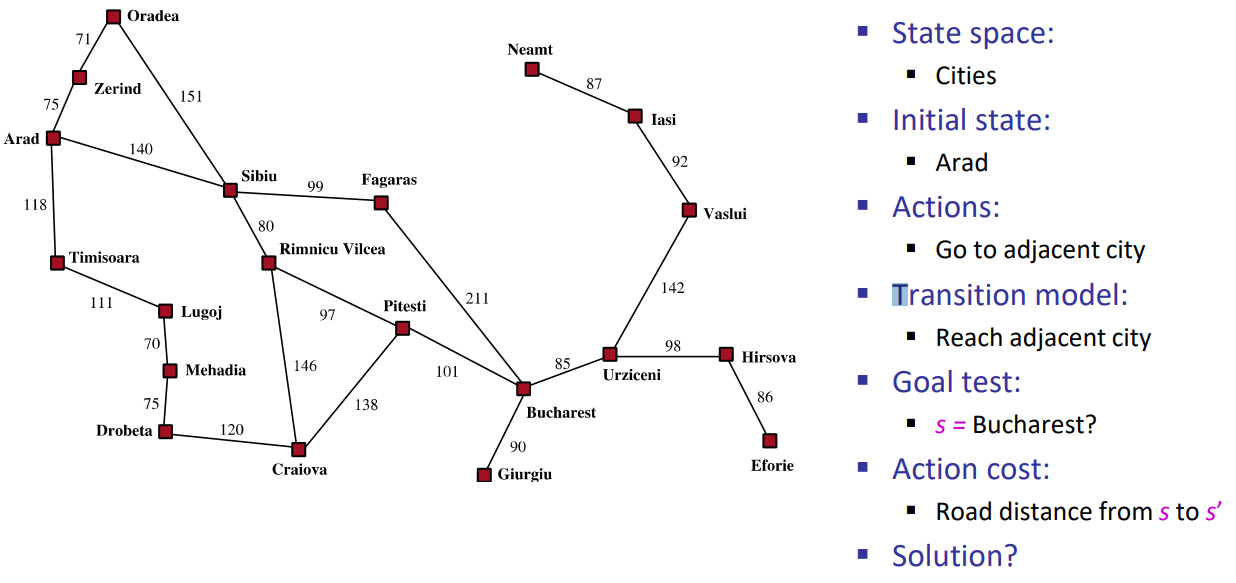
\includegraphics[width = 1\linewidth]{Images/21.PNG}
\end{center}
allora un algoritmo che l'agente può seguire per risolvere il problema è il seguente:
\begin{center}
    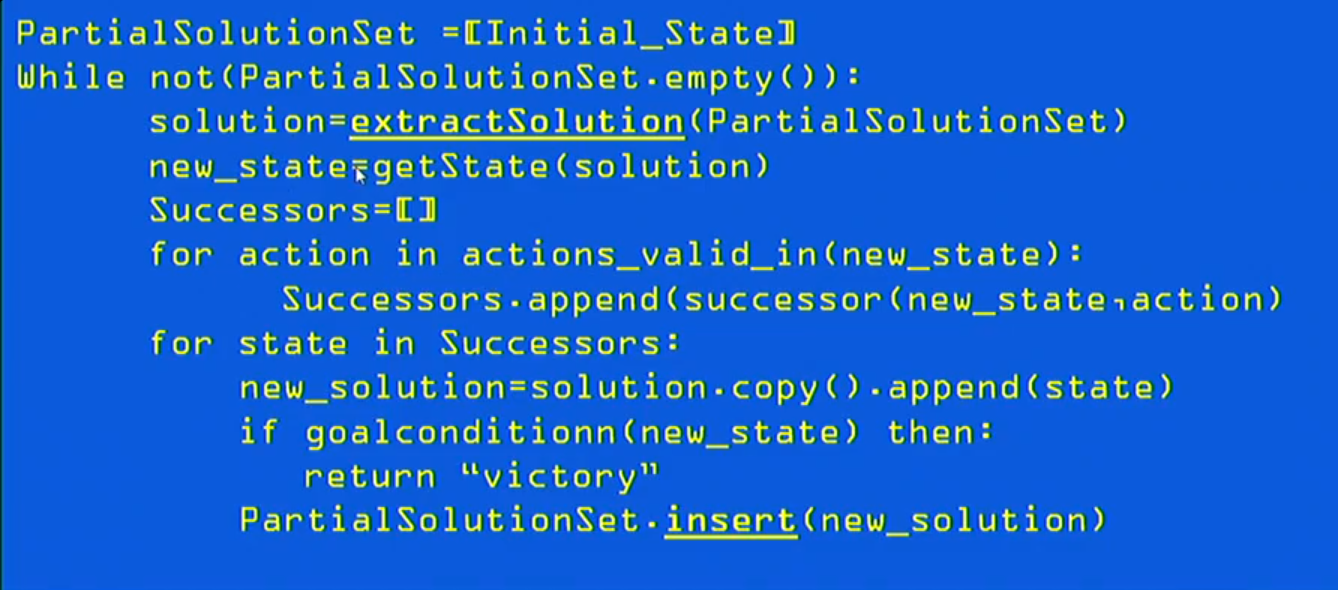
\includegraphics[width = 1\linewidth]{Images/22.PNG}
\end{center}
il modo in cui estraiamo una soluzione o ne aggiungiamo una nuova influenza l'efficienza dell'algoritmo.
Cambiando la struttura dati sottostante, viene inoltre cambiato \textbf{il comportamento dell'agente e le sue performance}.
Consideriamo ora un \textbf{agente basato su riflessi}; quando l'agente riceve un input $x$, allora esso effettua l'azione associata
a quell'input; quindi, se $f$ è la funzione che determina quale azione intraprendere, si può vedere l'agente in questo modo:
$$x \Rightarrow f \Rightarrow \textrm{singola azione } y \in \{-1, +1\}$$
Tuttavia, è piuttosto complesso costruire agenti di questo tipo per risolvere problemi di ricerca. Si preferisce quindi avere
agenti \textbf{basati sullo stato} che effettuano una simulazione interna e che siano in grado di \textbf{tenere traccia delle conseguenze delle proprie azioni} per arrivare alla soluzione:
$$x \Rightarrow f \Rightarrow \textrm{sequenza di azioni } (a_1, a_2, \dots)$$
tuttavia, abbiamo bisogno di questo tipo di agenti? Non potremmo risolvere questi problemi "senza pensare"?
\begin{itemize}
    \item Potremmo, in linea di principio, usare un agente basato su riflessi per risolvere un problema di ricerca? Potremmo creare una tabella di ricerca per determinare ogni nuovo stato a partire a seconda dell'azione intrapresa, ma solo sotto certe condizioni:
    \begin{itemize}
        \item L'informazione disponibile deve essere sempre sufficiente per poter effettuare una scelta
        \item Se non ci sono problemi di informazione, allora si potrebbe utilizzare una mappa degli stati per risolvere il problema di ricerca
    \end{itemize}
    \item Il problema principale a questo tipo di approccio è \textbf{il numero delle possibili configurazioni del problema}, visto che per ogni possibile configurazione è necessario avere una soluzione.
    \item Poiché le configurazione possono essere moltissime, allora la mappa rischia di essere enorme
\end{itemize}
Dobbiamo infine ricordare che quando si risolve un problema di ricerca, utilizziamo un \textbf{modello} che astrae le informazioni necessarie a risolverlo.
Per questo motivo, \textbf{i modelli, rispetto al mondo reale, risultano quasi sempre errati}, poiché tengono conto solamente delle informazioni rilevanti per risolvere il problema.
\subsection{Search Trees e algoritmi di ricerca}
Un modo molto semplice per codificare le soluzioni parziali ed effettuare delle scelte sono gli \textbf{alberi di ricerca} (search trees).
In questo tipo di struttura dati è:
\begin{itemize}
    \item Ogni nodo è uno \textbf{stato}
    \item La radice è lo \textbf{iniziale}
    \item I figli di ogni nodo corrispondono ai suoi \textbf{successori}
    \item Una \textbf{soluzione} è un \textbf{cammino} che dalla radice porta ad una foglia che soddisfa il "Goal Test"
\end{itemize}
\begin{center}
    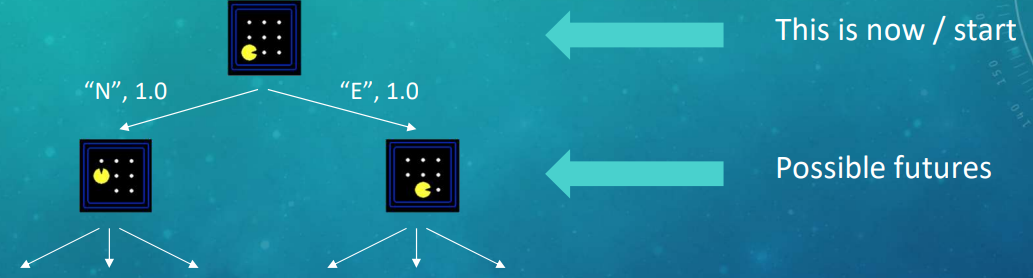
\includegraphics[width = 1\linewidth]{Images/23.PNG}
\end{center}
Un problema di questo approccio è che, a causa dell'elevato numero di stati, \textbf{non è quasi mai possibile espandere completamente l'albero di ricerca}.
Si rende quindi necessario lo sviluppo di approcci per ridurre i tempi computazionali.
\begin{center}
    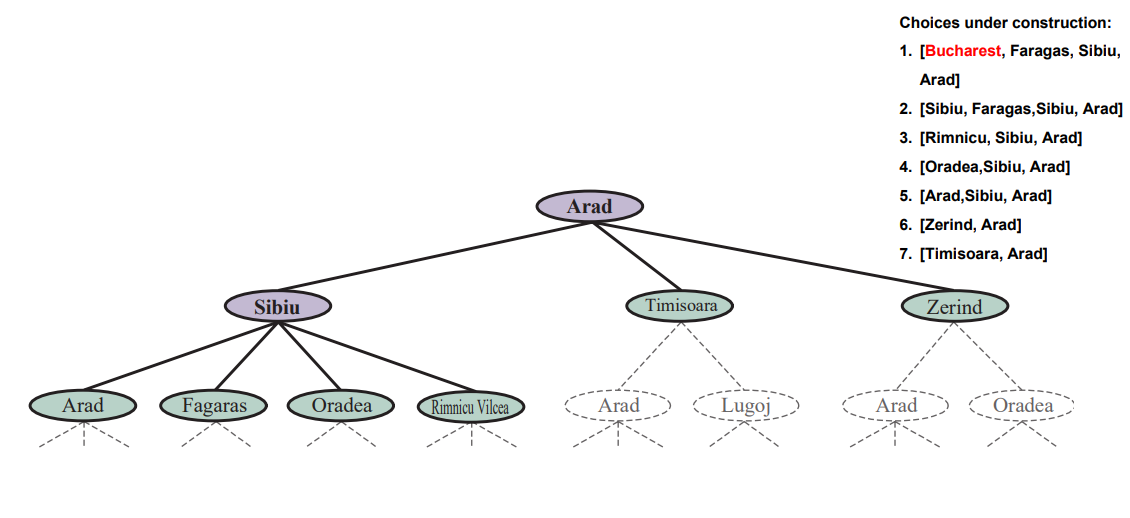
\includegraphics[width = 1\linewidth]{Images/24.PNG}
\end{center}
la differenza, quindi, tra i vari algoritmi di ricerca è il \textbf{modo in cui si sceglie di costruire ed esplorare l'albero}.
Un algoritmo generico per la \textbf{ricerca all'interno dell'albero è il seguente}:
\begin{center}
    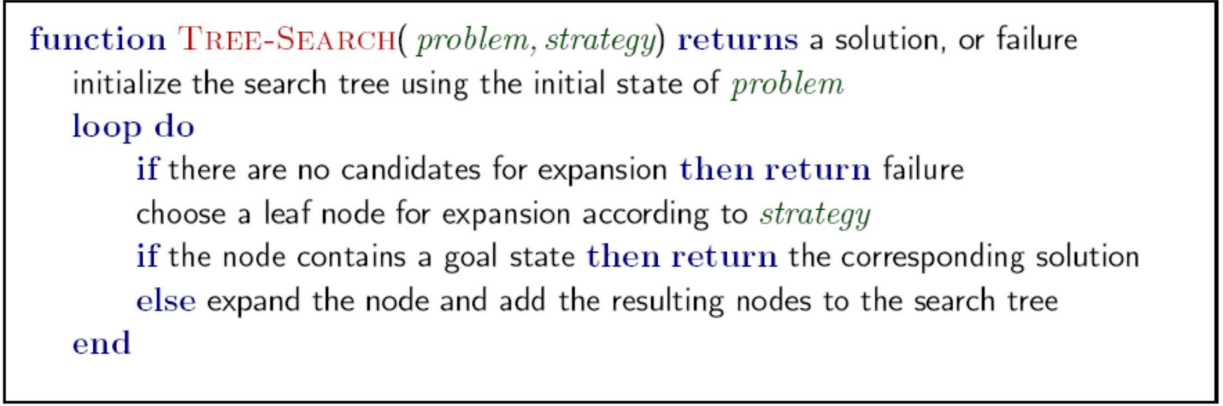
\includegraphics[width = 1\linewidth]{Images/25.PNG}
\end{center}
questa è un'implementazione basata sull'albero; la questione quindi diventa:
\begin{itemize}
    \item Quale nodo foglia espandere?
    \item Dobbiamo fare un controllo per stati ripetuti? (loop infiniti)
\end{itemize}
le proprietà di un algoritmo di ricerca generico sono le seguenti:
\begin{itemize}
    \item \textbf{Caratteristiche della ricerca}:
    \begin{itemize}
        \item \textbf{Completezza}: Garantisce di trovare una soluzione se esiste?
        \item \textbf{Ottimalità}: Garantisce di trovare il cammino di costo minimo?
    \end{itemize}
    \item Sia $b$ il \textbf{branching factor}, cioè il numero di azioni possibili per stato
    \item Sia $m$ (o $D$) la \textbf{massima profondità} a cui si può esplorare
    \item Le soluzioni possono essere a varie profondità
    \item Numero di nodi nell'intero albero? $$1 + b + b^2 + \dots + b^m = \mathcal{O}(b^m)$$
\end{itemize}
\begin{center}
    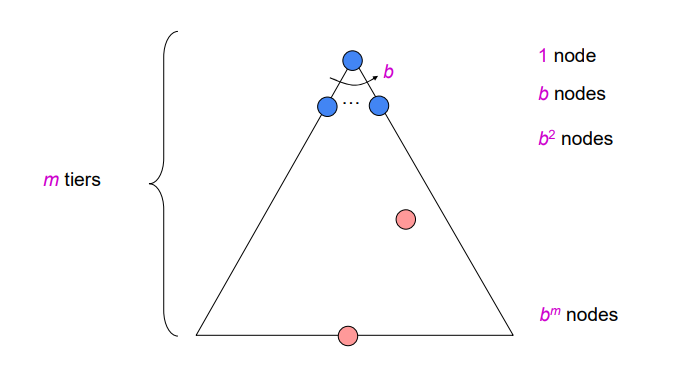
\includegraphics[width = 0.80\linewidth]{Images/29.PNG}
\end{center}
\subsubsection{Backtracking search}
Un primo algoritmo semplice che ci permette di trovare una soluzione nell'albero di ricerca
è il \textbf{Backtracking search}:
\begin{center}
    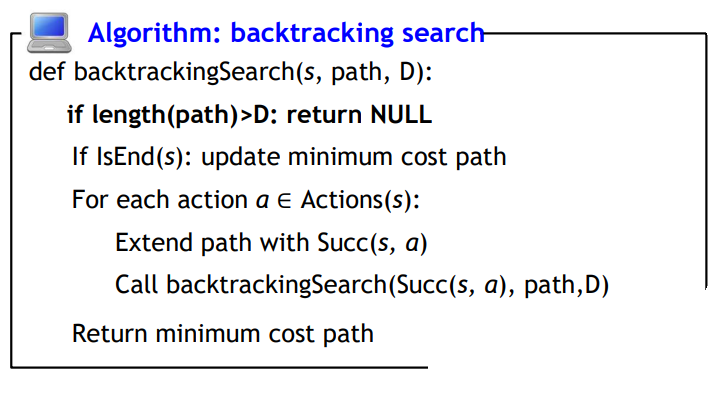
\includegraphics[width = 0.70\linewidth]{Images/26.PNG}
\end{center}
questo algoritmo espande sempre il primo nodo che non è stato espanso, fino ad arrivare ad una certa profondità.
Il limite alla profondità dell'albero permette di evitare che ci si possa fermare a causa di loop infiniti.
In questo modo, l'algoritmo \textbf{ricostruisce l'intero albero dei percorsi di lunghezza massima}, permettendo di poter effettuare
diverse domande sul nostro spazio degli stati. (es. percorso di lunghezza minima, percorso di costo minimo ecc...).
Lo svantaggio di questo algoritmo è che \textbf{deve espandere l'intero albero per trovare una soluzione} e non è detto che l'ultima soluzione trovata dall'algoritmo
\textbf{sia migliore di una soluzione trovata in precedenza}; tuttavia, questo tipo di algoritmo è estremamente flessibile, quindi si possono avere
delle condizioni arbitrarie che \textbf{impediscono all'algoritmo di continuare ad espandere l'albero in una certa direzione}.
Se abbiamo $b$ azioni possibili per stato, e un massima profondità $D$ di ricerca, allora i costi dell'algoritmo sono i seguenti:
\begin{itemize}
    \item \textbf{Memoria}: $\mathcal{O}(bD)$ (piccolo)
    \item \textbf{Tempo}: $\mathcal{O}(b^D)$ (enorme)
\end{itemize}
\subsubsection{Depth First Search}
A volte, non abbiamo condizioni complesse sul percorso ma, semplicemente, il valore di una foglia (quindi lo stato attuale) ci basta per capire
se la condizione di interesse è soddisfatta. Allora, in questo caso, possiamo usare un algoritmo di ricerca in profondità (DFS):
\begin{center}
    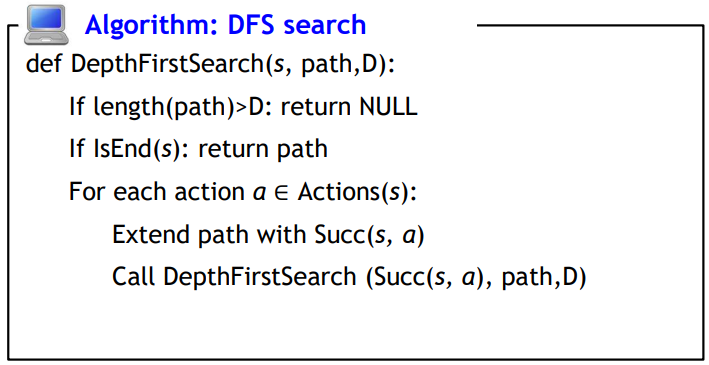
\includegraphics[width = 0.70\linewidth]{Images/27.PNG}
\end{center}
una volta che l'algoritmo trova una soluzione, \textbf{esso termina}.
L'algoritmo, durante la sua esecuzione, \textbf{tiene in memoria solamente le informazioni relative alla soluzione}.
\begin{center}
    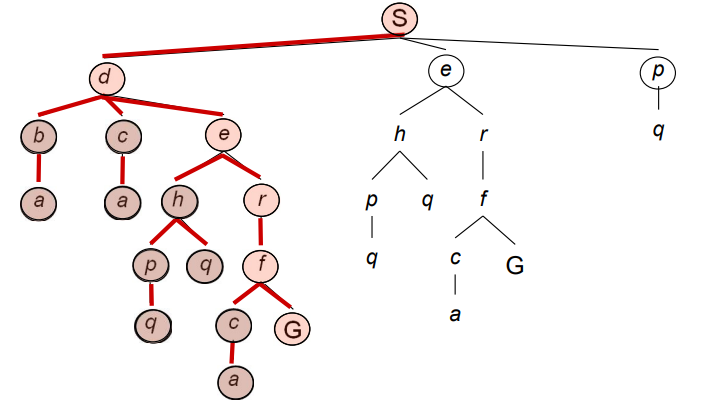
\includegraphics[width = 0.70\linewidth]{Images/28.PNG}
\end{center}
le uniche cose che bisogna memorizzare quando si effettua una DFS su un albero di ricerca sono quindi \textbf{quali nodi sono attivi nella soluzione attuale} e quali figli
di un certo nodo sono \textbf{ancora da esplorare}.
Le proprietà dell'algoritmo sono le seguenti:
\begin{itemize}
    \item Quali sono i nodi che la DFS espande?
    \begin{itemize}
        \item Espande alcuni nodi dell'albero fino ad una profondità $m$
        \item Potrebbe processare l'intero albero
    \end{itemize}
    \item \textbf{Completezza}: Poiché $m$ può essere infinito, prevenire dei cicli \textbf{potrebbe aiutare a trovare una soluzione}
    \item \textbf{Ottimalità}: L'algoritmo non è ottimale, dato che trova la \textbf{soluzione più a sinistra}, senza curarsi della profondità o del costo 
\end{itemize}
In termini di complessità, se si hanno $b$ decisioni per stato e la massima profondità permessa è $m$ si ha che:
\begin{itemize}
    \item \textbf{Spazio}: $\mathcal{O}(bm)$
    \item \textbf{Tempo}: $\mathcal{O}(b^m)$ nel caso peggiore, ma potrebbe ridursi molto se le soluzioni sono semplici da trovare
\end{itemize}
\begin{center}
    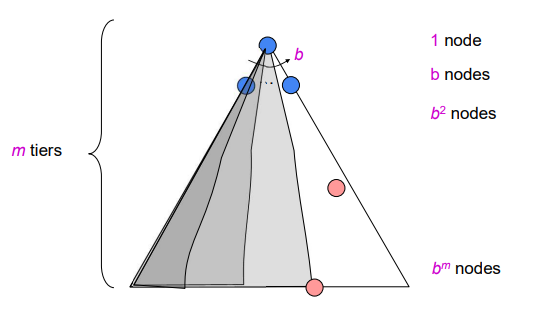
\includegraphics[width = 0.70\linewidth]{Images/30.PNG}
\end{center}
\subsubsection{Breadth First Search}
Una ricerca in ampiezza (BFS) andrà ad espandere \textbf{tutti i nodi dell'albero che si trovano allo stesso livello}. Così facendo, l'algoritmo
va a creare una \textbf{frontiera di nodi che devono essere ancora espansi}. Una volta terminati i nodi da espandere in un certo livello, l'algoritmo
passa ad espandere i nodi del livello successivo.
\begin{center}
    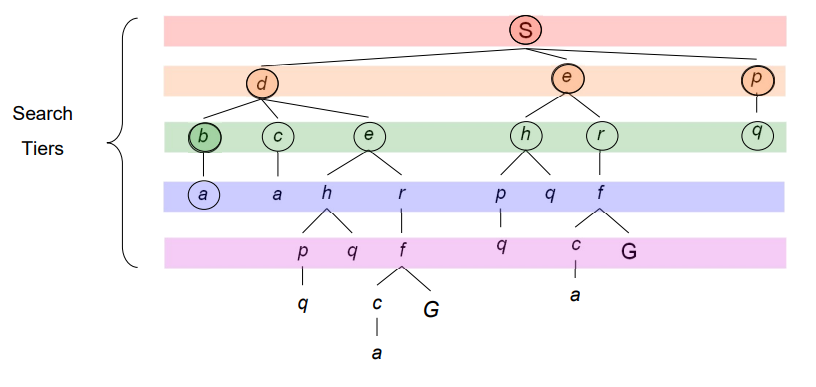
\includegraphics[width = 0.70\linewidth]{Images/31.PNG}
\end{center}
procedendo in questo modo, l'algoritmo \textbf{riesce a trovare la soluzione di costo minimo} (o quella che richiede meno passi).
Le proprietà della BFS sono le seguenti:
\begin{itemize}
    \item Quali nodi espande una BFS?
    \begin{itemize}
        \item Processa tutti i nodi sopra la soluzione meno in profondità. Sia questa profondità $s$
    \end{itemize}
    \item \textbf{Completezza}: Se $s$ è finito, allora di sicuro una soluzione esiste. L'algoritmo è completo
    \item \textbf{Ottimalità}: è ottimo solo se i costi dei cammini sono tutti \textbf{uguali}
\end{itemize}
\newpage
In termini di complessità, abbiamo che:
\begin{itemize}
    \item \textbf{Spazio}: $\mathcal{O}(b^s)$
    \item \textbf{Tempo}: $\mathcal{O}(b^s)$
\end{itemize}
\begin{center}
    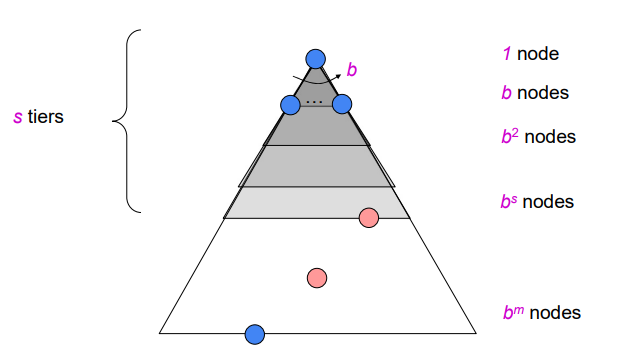
\includegraphics[width = 0.70\linewidth]{Images/32.PNG}
\end{center}
\subsubsection{DFS con approfondimento iterativo (DFS-ID)}
L'idea di questo algoritmo è di combinare la complessità spaziale di una DFS con la complessità
temporale di una BFS. L'algoritmo quindi esegue i seguenti passi:
\begin{itemize}
    \item Lancia una DFS con limite di profondità 1. Se non trovi soluzioni... 
    \item Lancia una DFS con limite di profondità 2. Se non trovi soluzioni... 
    \item Lancia una DFS con limite di profondità 3. Se non trovi soluzioni... 
    \item ...
\end{itemize}
\begin{center}
    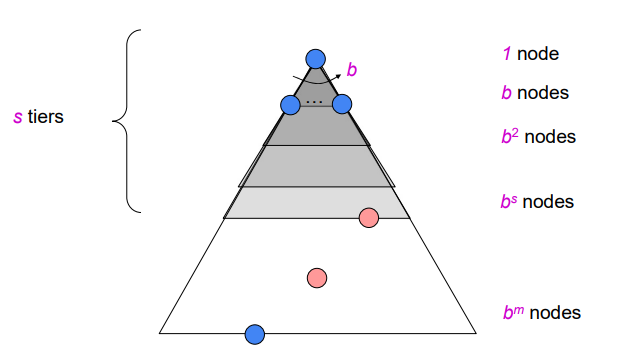
\includegraphics[width = 0.70\linewidth]{Images/32.PNG}
\end{center}
L'algoritmo, tuttavia, non è \textbf{estremamente ridondante?}
Generalmente, la maggior parte del lavoro avviene al \textbf{livello più in profondità esplorato},
quindi l'algoritmo non risulta ridondante. In termini computazionali, se si hanno $b$ possibili scelte per stato
e $s$ è la profondità della soluzione:
\begin{itemize}
    \item \textbf{Spazio}: $\mathcal{O}(s)$
    \item \textbf{Tempo}: $\mathcal{O}(b^s)$
\end{itemize}
ricapitolando:
\begin{center}
    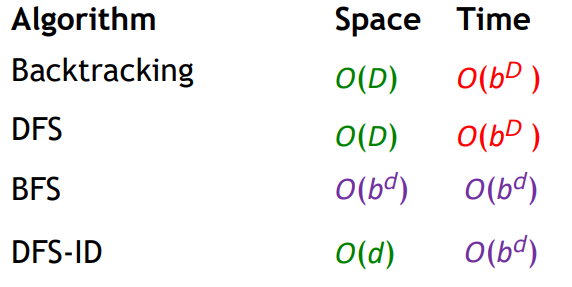
\includegraphics[width = 0.50\linewidth]{Images/34.PNG}
\end{center}
\subsubsection{Il problema della tigre}
Un esempio, molto presente in letteratura, è il cosiddetto "problema della tigre";
ed esso è un esempio di problema \textbf{non risolvibile con gli algoritmi che abbiamo visto fino ad adesso}.
\begin{center}
    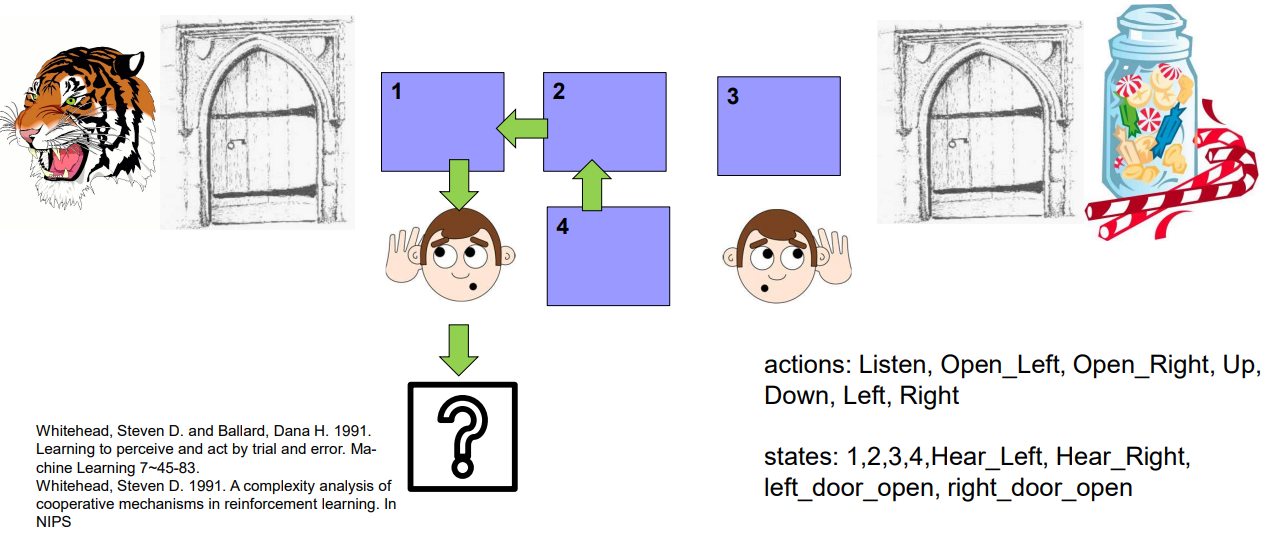
\includegraphics[width = 1\linewidth]{Images/35.PNG}
\end{center}
il problema ha la seguente traccia:
\begin{center}
    Ci si trova in un labirinto formato da stanze. Ogni stanza è collegata alle stanze adiacenti tramite una porta.
    Dietro ad ogni porta ci può essere una tigre oppure delle caramelle, le quali sono il nostro obbiettivo.
    Dopo ogni mossa, la tigre si può muovere in una delle stanze adiacenti a quella in cui si trova correntemente.
    Quale sequenza di azioni bisogna compiere per raggiungere l'uscita del labirinto?
\end{center}
l'agente non sa se dietro una determinata porta c'è la tigre oppure le caramelle; per scoprilo esso può \textbf{ascoltare e sentire se dietro ad una porta sente il rumore provocato dalla tigre}.
Se assumiamo che \textbf{ad ogni stato corrisponda lo stesso risultato} e che quindi una soluzione al problema sia \textbf{un'associazione tra uno stato ed un'azione}; allora in ogni stato possiamo assumere
di conoscere \textbf{quale azioni risolve il problema dato}. In questo caso, tuttavia, \textbf{questa assunzione è errata!} Se, per esempio, nello stato 1 decidiamo di \textbf{ascoltare}, allora abbiamo prodotto
l'associazione "nello stato 1, ascolta"; quindi, se più avanti nella risoluzione del problema torniamo allo stato 1, allora \textbf{ci troveremo ad ascoltare di nuovo}, poiché ad ogni stato viene associata un'azione.
Quindi, quando le conseguenze delle azioni non dipendono solamente da ciò che si può osservare in un determinato istante, non possiamo usare \textbf{gli algoritmi di ricerca che abbiamo visto fino ad ora per risolvere il problema}.
In questo caso bisognerebbe cambiare l'insieme degli stati in modo da \textbf{conservare l'informazione di "aver ascoltato la tigre"}.
Quando andiamo a definire lo spazio degli stati per un problema, ci sono diverse difficoltà da considerare poiché abbiamo la necessità 
che la conseguenza di un'azione dipenda solamente dallo stato in cui si compie l'azione.
Se lo spazio degli stati \textbf{non descrive tutte le informazioni necessarie per risolvere il problema, allora gli algoritmi di ricerca potrebbero entrare in un loop infinito} invece
che convergere alla soluzione.
\subsubsection{Grafo dello spazio degli stati}
Lo spazio degli stati e la funzione di transizione di un problema di ricerca possono anche essere rappresentati
\textbf{mediante un grafo orientato}, che prende il nome di \textbf{grafo dello spazio degli stati}
\begin{center}
    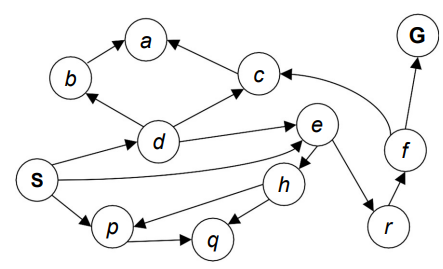
\includegraphics[width = 0.50\linewidth]{Images/36.PNG}
\end{center}
ogni nodo di un grafo dello spazio degli stati rappresenta uno \textbf{stato}, mentre ogni arco rappresenta \textbf{l'azione che dobbiamo intraprendere per passare da un certo stato ad un altro}.
In un grafo dello spazio degli stati \textbf{non ci possono essere stati duplicati!}
Come per l'albero di ricerca, è impossibile, per problemi interessanti, rappresentare in memoria l'intero grafo degli stati.
Un albero di ricerca \textbf{rappresenta l'insieme di percorsi e le soluzioni che sono state studiate fino a quel momento}; una soluzione del problema è quindi un \textbf{cammino dalla radice alla foglia il cui stato soddisfa le condizioni del problema}.
In certi casi, una rappresentazione a grafo dello spazio degli stati è molto più conveniente di un albero, il quale potrebbe risultare di profondità \textbf{infinita}
\begin{center}
    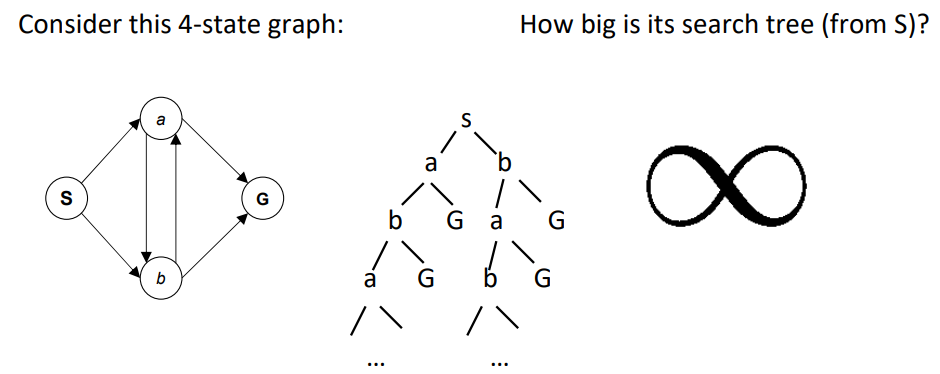
\includegraphics[width = 0.65\linewidth]{Images/37.PNG}
\end{center}
tendenzialmente quindi, un albero di ricerca ha più nodi di un grafo dello spazio degli stati.
\subsubsection{Il problema del costo}
Come abbiamo visto sopra, un problema di ricerca è anche caratterizzato dal \textbf{costo che ogni azione ha per essere intrapresa}.
Come sappiamo, una \textbf{soluzione} è una sequenza di azione che raggiunge uno stato che \textbf{superi il "goal test"} (quindi una soluzione arriva ad una configurazione accettabile del problema).
Una \textbf{soluzione ottima} è la soluzione \textbf{con il costo complessivo minore}.
Poiché diverse azioni, che portano in diversi stati, possono avere diversi costi; cosa può succedere quindi quando si cerca di costruire
un \textbf{cammino di costo minimo} su un grafo che presenta \textbf{degli archi con costo negativo}?
Se esiste un ciclo sul grafo che presenta archi di costo negativo, allora si rischia \textbf{che il cammino di costo minimo abbia costo $-\infty$}.
Per i prossimi algoritmi che presenteremo, assumeremo quindi che ogni arco abbia un costo \textbf{positivo}.
Prima di presentarli facciamo due ulteriori considerazioni:
\begin{itemize}
    \item Un algoritmo che effettua una BFS trova il cammino di costo minimo se e solo se i costi di ogni azione sono uguali
    \item Un algoritmo che effettua una DFS trova il cammino di costo minimo se e solo se i costi di ogni azione sono nulli
\end{itemize}
\subsubsection{Uniform Cost Search (UCS)}
In questo algoritmo, si procede ad esplorare il nodo che ha \textbf{costo minore dall'origine}.
\begin{center}
    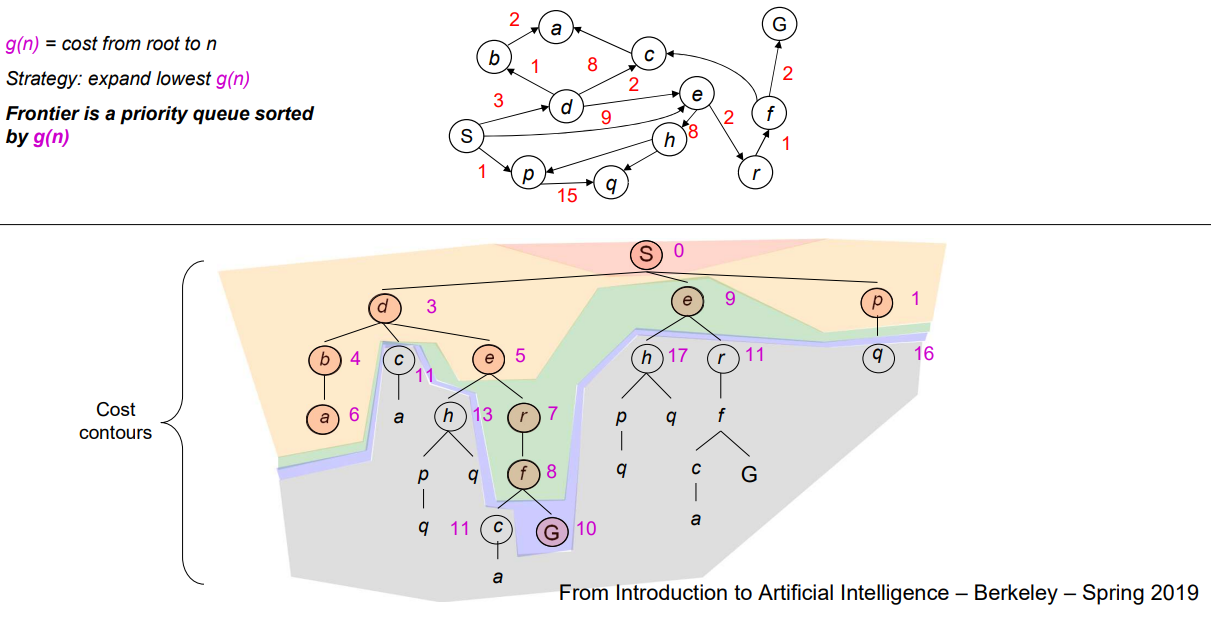
\includegraphics[width = 1\linewidth]{Images/38.PNG}
\end{center}
un implementazione di questo algoritmo è quindi la seguente:
\begin{center}
    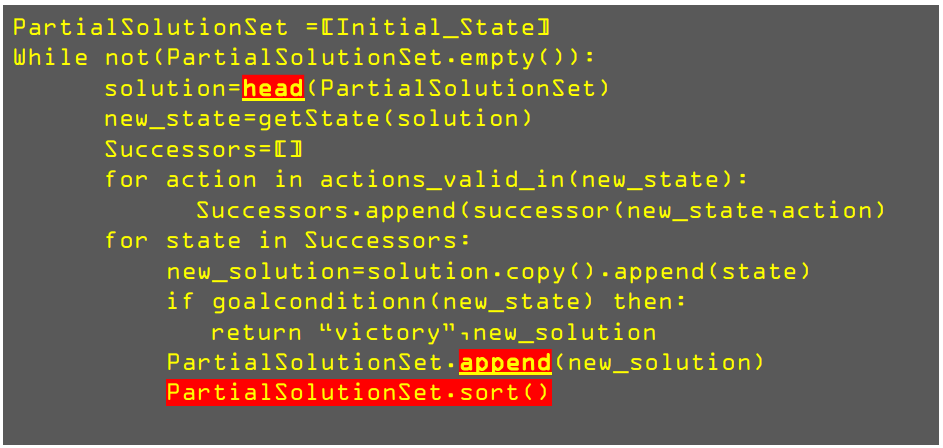
\includegraphics[width = 0.85\linewidth]{Images/39.PNG}
\end{center}
questo algoritmo ha le seguenti proprietà:
\begin{itemize}
    \item Quali nodi espande l'algoritmo?
    \begin{itemize}
        \item Espande tutti i nodi con \textbf{costo minore rispetto alla soluzione meno costosa!}
        \item Se la soluzione costa $C^*$ e gli archi hanno un costo di almeno $\varepsilon$, allora "la profondità effettiva" della soluzione meno costosa è $C^*/\varepsilon$.
    \end{itemize}
    \item \textbf{Completezza}: Assumendo che $C^*$ è finito e $\varepsilon > 0$, allora si!
    \item \textbf{Ottimalità}: L'algoritmo è ottimale
\end{itemize}
In termini computazionali, si ha che, se $b$ è il numero di azioni possibili in ogni stato:
\begin{itemize}
    \item \textbf{Spazio}: $\mathcal{O}(b^{C^*/\varepsilon})$
    \item \textbf{Tempo}: $\mathcal{O}(b^{C^*/\varepsilon})$
\end{itemize}
\begin{center}
    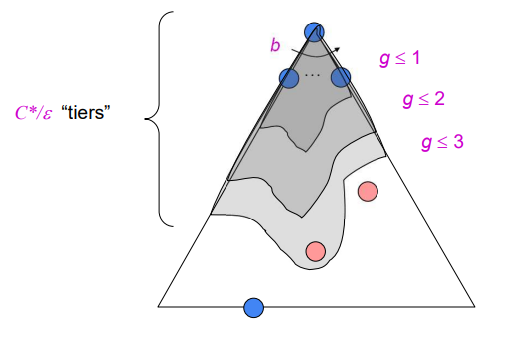
\includegraphics[width = 0.55\linewidth]{Images/40.PNG}
\end{center}
Enunciamo il teorema di \textbf{correttezza} per questo algoritmo:
\begin{Teorema}[Correttezza di UCS]
    Quando uno stato $s$ viene rimosso dalla frontiera e posto tra i nodi esplorati, la sua priorità è $PastCost(s)$, cioè il minimo costo di $s$
\end{Teorema}
\begin{Dimostrazione}
    Se $s$ viene scelto, allora è il nodo che ha \textbf{costo minimo sulla frontiera}; quindi ogni altro cammino ad $s$ sarà più costoso, se i costi sono positivi.
    Per ogni nodo $u$ nella frontiera, si ha che:
    $$PastCost(s) \leq PastCost(u) \leq PastCost(u) + Cost(u,s)$$
    \begin{center}
        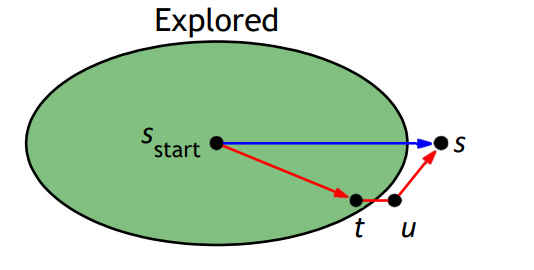
\includegraphics[width = 0.55\linewidth]{Images/41.PNG}
    \end{center}
\end{Dimostrazione}
Tutti gli algoritmi che abbiamo visto fino ad ora sono \textbf{uguali} tranne per \textbf{la gestione dei nodi sulla frontiera}:
\begin{itemize}
    \item Concettualmente, tutte le frontiere sono code di priorità (cioè, collezioni di nodi a cui viene attaccata una certa priorità)
    \item Praticamente, per DFS e BFS, si può evitare l'overhead di $log(n)$ dato da una priority queue usando stack e code
    \item Si può addirittura implementare una variante che prende in input "oggetto di accodamento" (variabile)
\end{itemize}
\subsubsection{Ricerca informata}
Il problema principale di UCS è che \textbf{esplora l'albero degli stati in ogni direzione}; quindi non tiene conto di nessuna informazione
riguardante la \textbf{posizione dell'obbiettivo all'interno dell'albero}.
\begin{center}
    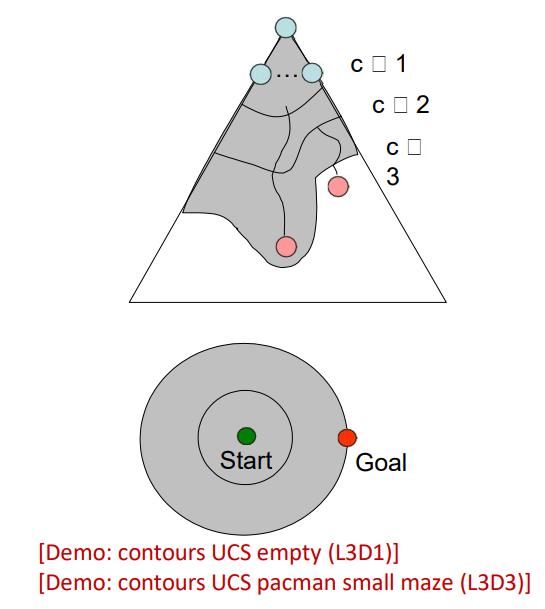
\includegraphics[width = 0.45\linewidth]{Images/42.PNG}
\end{center}
per velocizzare il processo di ricerca, dobbiamo quindi \textbf{guidare la ricerca verso l'obbiettivo}, invece che cercare in tutte le direzioni possibili.
Questo tipo di ricerca viene detto \textbf{ricerca informata}
\begin{center}
    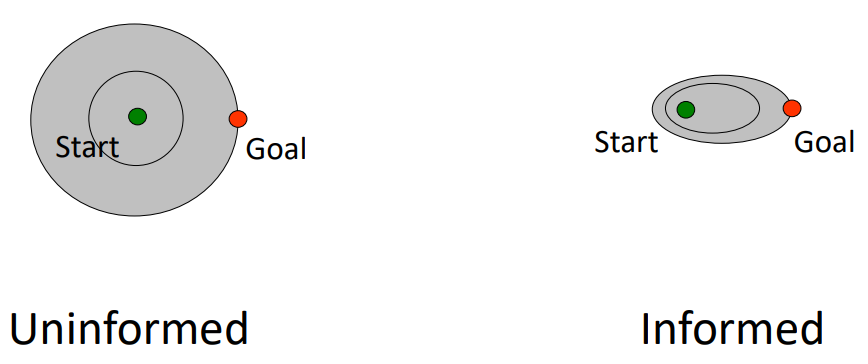
\includegraphics[width = 0.45\linewidth]{Images/43.PNG}
\end{center}
per poter far questo, abbiamo bisogno di inserire più informazione.
In questo caso, tuttavia, l'informazione aggiuntiva non riguarda delle caratteristiche dell'oggetto ma è una \textbf{semplice funzione euristica} che
indica "quanto è facile raggiungere lo stato un obbiettivo da un certo stato".
Queste funzioni euristiche sono \textbf{funzioni dell'obbiettivo}, quindi, per ogni obbiettivo da raggiungere, necessitiamo di una funzione euristica.
Quindi, \textbf{un euristica} è:
\begin{itemize}
    \item Una \textbf{funzione} che \textit{stima} quanto vicino è uno stato all'obbiettivo
    \item Ogni euristica è progettata per un particolare problema di ricerca
    \item Esempi: Manhattan Distance, Euclidean Distance for pathing ecc...
\end{itemize}
Se l'agente impara una certa funzione euristica per un certo obbiettivo; se l'obbiettivo cambio sarà necessario apprendere
una nuova euristica. Un euristica, per funzionare, deve però \textbf{effettuare previsioni minori del valore reale}, cioè deve sottostimare
il costo di raggiungere l'obbiettivo rispetto al costo reale.
\subsubsection{Greedy Search}
Uno degli approcci che utilizza le euristiche viene chiamato \textbf{greedy search}.
L'algoritmo andrà ad esplorare il nodo \textbf{che sembra essere più vicino all'obbiettivo}
\begin{center}
    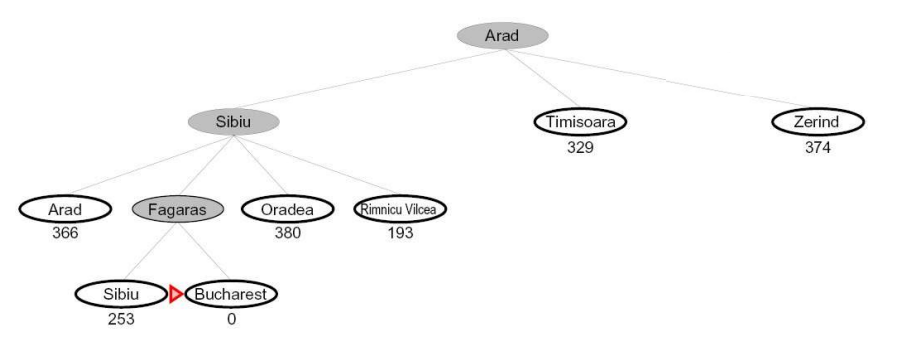
\includegraphics[width = 1\linewidth]{Images/44.PNG}
\end{center}
l'algoritmo è quindi simile ad UCS, ma al posto di esplorare il nodo che ha costo minimo rispetto all'origine,
\textbf{esplora invece il prossimo nodo che ha un costo atteso, quindi un'euristica minima, verso l'obbiettivo}.
La strategia dell'algoritmo è quindi quella di espandere il nodo che \textbf{l'euristica valuta come più vicino all'obbiettivo} (quindi il migliore tra i nodi da esplorare).
L'euristica in questo caso offre, \textbf{per ogni stato dell'albero}, una \textbf{stima della distanza dall'obbiettivo più vicino}.
\begin{center}
    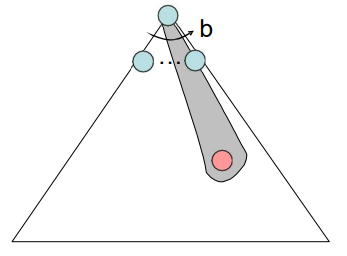
\includegraphics[width = 0.40\linewidth]{Images/45.PNG}
\end{center}
L'algoritmo tuttavia, \textbf{in presenza di un euristica non ottimale}, fatica nel trovare effettivamente una soluzione ottima \textbf{poiché esso non tiene conto del costo totale per raggiungere ogni nodo a partire dalla radice} ma
considera solamente il costo \textbf{per passare da un nodo all'altro}.
\begin{center}
    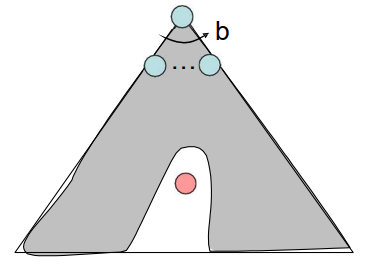
\includegraphics[width = 0.40\linewidth]{Images/46.PNG}
\end{center}
\subsubsection{$A^*$ Search}
L'algoritmo di ricerca $A^*$ combina gli algoritmi UCS e Greedy Search.
Per farlo, assegna ad ogni nodo dell'albero un numero ottenuto sommando i costi del percorso seguito per arrivare fino a quel nodo e la stima del costo che
l'euristica prevede per arrivare all'obbiettivo da quel nodo.
Siano quindi:
\begin{itemize}
    \item $g(n)$ il costo per arrivare dalla radice al nodo $n$
    \item $h^*(n)$ il costo ottimale per arrivare da $n$ all'obbiettivo più vicino
\end{itemize}
L'idea alla base di $A^*$ è quindi la seguente:
\begin{itemize}
    \item Si espande un nodo $n$ che ha maggiore probabilità di essere su un cammino ottimale verso l'obbiettivo
    \item Si espande un nodo $n$ tale che il costo della migliore soluzione che passa per $n$ sia ottimale
    \item Si espande un nodo $n$ con il minor valore di $g(n) + h^*(n)$ 
    \item Solo in rari casi sappiano quanto vale $h^*(n)$, tuttavia potremmo avere una sua \textbf{approssimazione euristica} $h(n)$
    \item $A^* =$ ricerca su un albero con una coda di priorità ordinata rispetto a $f(n) = g(n) + h(n)$
\end{itemize}
\begin{center}
    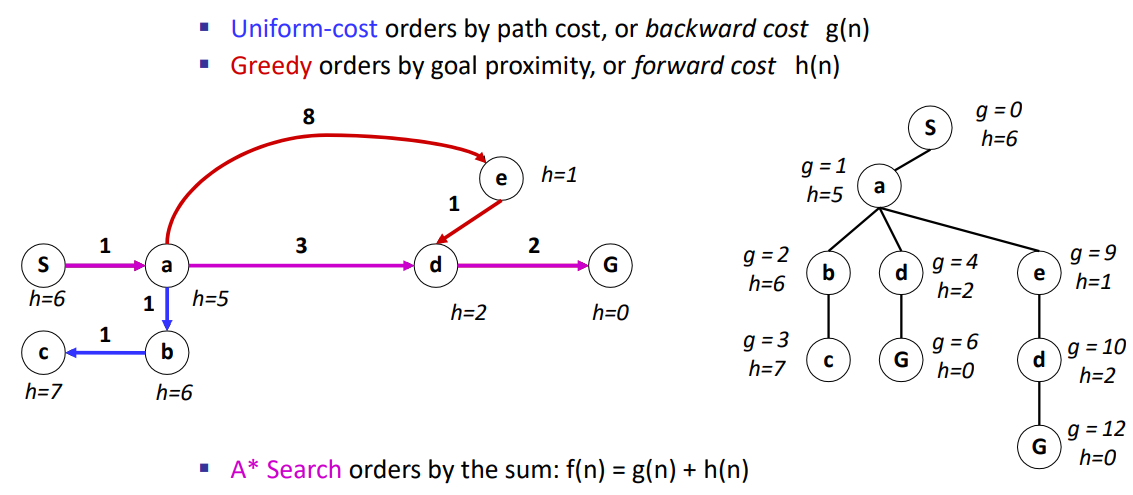
\includegraphics[width =1\linewidth]{Images/47.PNG}
\end{center}
Per fare in modo che \textbf{$A^*$ sia ottimo}, abbiamo bisogno che l'euristica sia \textbf{ottimista rispetto al costo reale}.

% 1:40:46






\end{document}
